\documentclass[11pt,dvipsnames]{scrreprt}%oldschool: report

\usepackage[utf8]{inputenc}
\usepackage{ngerman}
\usepackage{fullpage} % kleinere Ränder

\usepackage{comment} % für größere comments: \begin{comment} ... \end{comment}

% *** für eingefügte (pdf-)Grafiken
\usepackage[pdftex]{graphicx} 
%\pdfminorversion=6
% ***

\usepackage{float}
\restylefloat{figure}

\usepackage{enumerate} %für geschachtelte Aufzählungen


\linespread{1.25}
\usepackage{amsmath} %Matheformeln usw.
\usepackage{amssymb} %mathfrak

\usepackage[bookmarks=true]{hyperref} % hyperrefs aktivieren
\setcounter{secnumdepth}{3} %Numerierung bis Tiefe 3, also ab \paragraph ohne

% *** java listings
\usepackage{xcolor,luximono,listings}
\usepackage{listings}
\lstloadlanguages{PYTHON,SQL,XML,JAVA}
\usepackage{courier} % courier schrift
\lstset{
	language=Java, 
	basicstyle=\ttfamily, 
	tabsize=4,
	literate= {Ö}{{\"O}}1 {Ä}{{\"A}}1 {Ü}{{\"U}}1 {ß}{{\ss}}2 {ü}{{\"u}}1
 	{ä}{{\"a}}1 {ö}{{\"o}}1
}
% end listing ***

% *** requirements commands definition
% use \initReqgrp{<group-ref>} to set group
% use \req{<title>}{<requirement-ref>} to set a main requirement (label inclusive)
% use \subreq{<title>}{<subrequirement-ref> to set a sub requirement (label inclusive)

\gdef \reqGrp{x}% 										requirement group prefix
\gdef \reqMain{x}% 										requirement reference shortcut
\gdef \reqSub{x}% 										requirement reference shortcut
\newcounter{cntReqGrp}% 								requirement group counter
\newcounter{cntReq}[cntReqGrp]% 						main requirement counter
\newcounter{cntSubReq}[cntReq]% 						sub requirement counter
\newcommand{\reqPrefix}{/}
\newcommand{\reqPostfix}{/}
\renewcommand{\thecntReq}{\reqPrefix\reqGrp-\arabic{cntReq}\reqPostfix}% 		set output or cntReq
\renewcommand{\thecntSubReq}{\reqPrefix\reqGrp-\arabic{cntReq}.\arabic{cntSubReq}\reqPostfix}% set output of cntSubReq
\newcommand{\req}[2] {% 								define new requirement, input: title, reference shortcut
	\refstepcounter{cntReq}% 								update counter
	\gdef \reqMain{#2}% 								update requirement reference
	\thecntReq\  #1% 									set output \end{reqtxt} label text
	\label{req:\reqGrp:#2}% 							set label 
}

\newcommand{\subreq}[2] {% 								define new sub requirement, input: title, reference shortcut
	\refstepcounter{cntSubReq}% 							update counter
	\gdef \reqSub{#2}% 									update requirement reference
	\thecntSubReq\  #1% 			set output text 
	\label{req:\reqGrp:\reqMain:\reqSub}% 				set label
}

\newcommand{\initReqgrp}[1] {% 							init new requirement group, input: prefix
	\gdef \reqGrp{#1}% 									overwrite variable reqgrp
	\refstepcounter{cntReqGrp}% 						update group counter
}
% *** end requirements commands


% *** shortcuts
\def \arc{ARC}
\def \ci{Christoph Piechula}
\def \cii{Christoph Cwelich}
\def \ciii{Christopher Pahl}
\def \eddy{Eduard Schneider}
\def \flo{Florian Bauer}
\def \sab{Sabrina Biersack}

% ***

%*** title etc.
\title{Dokumentation\\
Praktikum Software Entwicklung }
\author{Dozent: Prof. Dr. Richard Göbel \\
Beteiligte Studenten: \\
\sab, \\ \flo, \\ \eddy, \\ \ci, \\ \cii, \\ \ciii
}
\date{\today}
%***

%newcommands
%\newcommand{\neuesKommando}{Was zu tun ist}
\newcommand{\todo}[1]{\Huge{TODO: #1}}
\newcommand{\code}[1]{\lstinline{#1}}
\newcommand{\liable}[1]{Verantwortlich: #1 \\}
\begin{document}

\maketitle

\tableofcontents

\part{Spezifikation}
\chapter{Übersicht}
Über einen konfigurierbaren Crawler können Inhalte von Webseiten bis zu einer bestimmten Tiefe
aus dem Internet in ein Archiv geladen werden. Da dies parallelisiert erfolgen soll,
müssen die Daten nach dem Herunterladen von temporären Verzeichnissen in das gemeinsame
Archivverzeichnis synchronisiert werden. Der aus der URL extrahierte Pfad der Dateien wird
dabei auf das Archiv abgebildet, wobei jede Datei in einen eigenen Archivordner verschoben wird.\\

Beim Crawlvorgang werden zusätzlich Metadaten der heruntergeladenen Dateien erstellt. 
Diese werden in einer Datenbank und als XML-Datei im jeweiligen Archivordner gespeichert.
Die Datenbank soll dabei wieder aus den XML-Daten rekonstruierbar sein. \\ 

Außerdem sollen Filter eingehängt werden können, die bereits in den TMP-Ordnern ungültige Dateien löschen.
Über eine Java-Schnittstelle kann anschließend wieder auf die Daten zugegriffen werden.
Hierzu müssen sich Clients über eine vorgegebene Schnittstelle beim Textarchiv anmelden.
Die Clients werden anschließend bei Änderungen oder neuen Einträgen benachrichtigt und können sich selbstständig über die Schnittstelle einen beliebigen Stand der Daten herunterladen und an Analysetools weitergeben.
Dabei sollen auch neue Dateien den Archivordnern hinzugefügt werden können.
Ebenso sollen die oben genannten XML-Daten um neue Nodes erweiterbar sein.
Zu Vorführzwecken wird ein Testanalysetool erstellt.


 

\chapter{Datenmodell der Metadaten} \label{spec:model}
An dieser Stelle wird bereits ein vereinfachtes Datenmodell festgelegt, welches
später auf Datenbank und XML-Daten umgesetzt wird und zentrale Metadaten über HTML-Seiten erfassen soll. 

Für jede HTML-Datei wird dabei ein solcher Satz von Metadaten angelegt.
Die Metadaten sollen vor allen Dingen Such- und Sortieraufgaben erleichtern. 

\begin{table}[h]
\centering
\begin{tabular}{|l|l|l|}	
	\hline
	Name 		& Datentyp 				& Beschreibung \\
	\hline
	URL 		& String 				& Original URL der HTML-Datei\\
	Titel 		& String 				& Soweit vorhanden wird der Titel der Seite \\ 
	 			& 						& gespeichert \\ 
	Archivpfad 	& String 				& Dateipfad des \htmlarc-Ordners im Webarchiv \\
	Crawlzeit 	& Timestamp oder 		& Zeitpunkt des Crawls \\
				& Integer (UTC in ms) 	&  \\
	Commit Tag 	& String 				& Der Committag dient zum Wiederauffinden \\
	 			& 						& in der Versionsverwaltung. \\ 
				& 						& Der Tag setzt sich aus Domainnamme und \\
				& 						& dem Zeitpunkt des Crawlvorgangs zusammen.\\
	\hline
\end{tabular}
\caption{Metadaten}
\end{table}


\chapter{Anforderungen}
Im folgenden sind die Anforderungen an die Software spezifiziert. Soweit möglich wurden
die Anforderungen schon in einzelne Komponenten und Module gegliedert. Eine grobe Übersicht gibt auch Diagramm
im Abschnitt \ref{spec:dia:moduls}.

Alle Anforderungen werden mit einer Kennnummer in der Form 
\[ \text{\reqPrefix}<Gruppenprefix> . <Anforderungsnummer> [. <Unternummer> ]\text{\reqPostfix} \]
gekennzeichnet, damit diese später wieder referenziert werden können.

\section{Crawlermodul}
\initReqgrp{Cr}
Dieses Modul soll als eigenständiger Prozess laufen und in regelmäßigen Abständen Crawlvorgänge starten
und die Daten in das Archiv schreiben.

\subsection{Steuerung}
\begin{description}
    \label{spec:conf}
	\item [\req{Config-file}{conf}]
		Die Steuerung des bzw. der Crawler erfolgt über eine Config-Datei.
		Ist die Config-Datei nicht vorhanden oder kann sie nicht gelesen werden,
        so werden hart codierte Werte verwendet.
		Es können folgende Parameter eingestellt werden:
		\begin{description}
			\item [\subreq{Suchtiefe}{depth}]
				Suchtiefe bis zu der Links gefolgt werden soll.
			\item [\subreq{Crawlintervall}{interval}]
				Zeitintervalle zwischen den Crawlvorgängen.
			\item [\subreq{Maximale Instanzen}{maxInst}]
				maximale Anzahl der gleichzeitig gestarteten Crawlerinstanzen.
			\item [\subreq{Filtereinstellungen}{filter}]
				Liste von Verwendeten Ausschlussfiltern und deren Modulpfad.
			\item [\subreq{Berücksichtigung von robots.txt}{robotsTxt}]
				Man kann einstellen, ob robots.txt berücksichtigen werden soll.
			\item [\subreq{User Agent}{userAgent}]
				Man kann einen User Agent festlegen.
			\item [\subreq{URL Liste}{urllist}]
                Ein Pfad zu einer Liste mit zu crawlenden URLs ist definiert.
			\item [\subreq{Archiv root Pfad}{root}]
				Es wird der Wurzelpfad für die Archivordner festgelegt.
		\end{description}
	\item [\req{Kommandozeileninterface}{cmd}]
		Optional können beim Start mittels Kommandozeile zusätzliche Parameter übergeben werden.
		\begin{description}
			\item [\subreq{Überschreiben}{overwrite}]
				Werte aus dem Config-file werden damit überschrieben.
			\item [\subreq{DB-Recovery erzwingen}{recover}]
				Es kann ein Datenbank-Recovery erzwungen werden. Siehe auch \ref{req:Db:recovery}
		\end{description}
\end{description}

\subsection{Ausführung des Crawlvorgangs} \label{spec:crawler:exec}
\begin{description}
	\item [\req{Start in Intervallen}{startInterval}]
		Der Crawlvorgang wird immer wieder nach einem gemäß \ref{req:conf:interval} festgelegtem
		Interval neu in Gang gesetzt. 
	\item [\req{Parallelität}{concurrent}]
		Die Ausführung der Crawlvorgänge soll parallel durchgeführt werden.
	\item [\req{URL-Queue}{urlqueue}]
		Alle aus \ref{req:Cr:conf:urllist} werden in eine Warteschlange geschrieben.
	\item [\req{Instanziierung}{instance}]
				Für die Crawlerinstanzen wird ein externes Tool verwendet: WGET
		\begin{description}
			\item [\subreq{Temporäre Ordner anlegen}{createTmp}]
				Für jede Crawlerinstanz wird ein eigenes temporäres Verzeichnis zum Speichern
				der Downloads angelegt. Im folgenden mit TMP abgekürzt.
			\item [\subreq{Start}{start}]
				Es werden solange Crawlerinstanzen mit URLs als Startpunkt aus der URL-Queue erzeugt,
				bis diese leer ist. 
			\item [\subreq{maximale Instanzen}{maxInst}]
				Wird die Obergrenze an maximal erzeugbaren Instanzen erreicht 
				(siehe \ref{req:Cr:conf:maxInst}),
				wird immer solange mit dem Erzeugen neuer Instanzen gewartet,
				bis die nächste	Crawlerinstanz fertig ist.
			\item [\subreq{Domain-Überschneidungen}{domain-intersection}]
				Um Überschneidungen zu vermeiden, werden Domainnamen anderer Instanzen ausgeschlossen.
		\end{description}
	\item [\req{Crawlen}{crawl}]
		Jede gestartete Instanz beginnt nun den Crawlvorgang.
		\begin{description}
			\item [\subreq{Herunterladen}{download}]
				Jede Instanz kopiert die heruntergeladene Dateien 
				der Seite in ein temporäres Verzeichnis je Crawlerinstanz.
			\item [\subreq{Ordnerstruktur}{structure}]
				Dabei wird die online vorhandene URL-Pfadstruktur der Dateien 
				auf das Dateisystem abgebildet.
				Je Domain wird dadurch ein Hauptverzeichnis im TMP-Ordner erzeugt.
		\end{description}
	\item [\req{Bereinigung}{clean}]
		In diesem Teil werden die heruntergeladenen Ordner bereinigt,
		also leere Ordner gelöscht.
	\item [\req{Normalisierung}{normalize}]
		Durch die Normalisierung werden die Dateien auf eine dem Archiv entsprechende Struktur gebracht.
		\begin{description}
			\item [\subreq{Datei umbenennen}{rename}]
				Das File wird in ''data.<Endung>'' umbenannt. 
			\item [\subreq{Archivordner erzeugen}{createArc}] 
				Es wird ein Archivordner (im Folgenden kurz \arc\ genannt) 
				mit dem Namen der Datei (inklusive Dateiendung) 
				erzeugt.
			\item [\subreq{Datei verschieben}{move}]
				Die data-Datei wird in das soeben erzeugte \arc\ verschoben.
		\end{description}
	\item [\req{Extraktion der Metadaten}{metaextract}]
		In diesem Vorgang werden die im Datenmodell (Abschnitt \ref{spec:model}) 
		definierten Metadaten 
		aus der Datei extrahiert und zwischengespeichert. 
		\begin{description}
			\item [\subreq{url}{url}]
				Die Original-URL wird aus dem aktuellen Ordnerpfad abgeleitet.
			\item [\subreq]{title}{title}
				Da das title-feld generisch gehalten ist, 
				muss die Extraktionsschnittstelle so erweiterbar sein,
				dass verschiedene Formate unabhängig behandelt werden können. 
			\item [\subreq{HTML-title}{htmltitle}]
				Es wird eine Titelextraktionsmethode
				für HTML-Dateien implementiert, die
				nach dem Titel-Tag sucht.
			\item [\subreq{mimeType}{mimeType}]
				Der MIME-Typ der Datei wird mit einer geeigneten Maßnahme ermittelt.
			\item [\subreq{path}{path}]
				Es wird der aktuelle absolute Ordnerpfad auf das \arc gespeichert.
			\item [\subreq{domain}{domain}]
				Der Name der Domain wird aus der dem Domainordnernamen kopiert.
			\item [\subreq{createTime}{createTime}]
				Das Erzeugungsdatum der Datei wird ermittelt.
		\end{description}
	\item [\req{Filterung}{filter}]
		Für alle Dateien wird eine Liste von Filtern durchlaufen.
		Jeder Filter prüft, ob die Datei behalten oder verworfen werden soll.
		Verworfene Dateien werden sogleich gelöscht.
	\item [\req{commitTime speichern}{commitTime}]
		Der Startzeitpunkt wird sofort nach dem Beginn des Crawlvorgangs zwischengespeichert.
		Siehe auch Abschnitt \ref{spec:model}.
	\item [\req{Erzeugung von XML-Dateien}{xml}]
		Die zwischengespeicherten Metadaten werden in XML-Metadateien 
		(siehe auch Abschnitt \ref{spec:xml}) 
		geschrieben und jeweils im zugehörigen \arc\ als ''data.xml'' gespeichert. 
	\item [\req{Synchronisation}{sync}]
		Die vorbereiteten Daten in den TMP-Ordnern werden nun in das vorhandene Archiv synchronisiert 
		(mit RSYNC). (Siehe auch Abschnitt \ref{spec:filearchive})
		\begin{description}
			\item [\subreq{Update}{update}]
				Veraltete \arc s werden komplett durch die neuen ersetzt
				(und dadurch von der Versionierung in einen älteren Branch verschoben).
		\end{description}
	\item [\req{Datenbankaktualisierung}{dbupdate}]
		Die Datenbank wird nun mithilfe der zwischengespeicherten Metadaten aktualisiert.
\end{description}

%\begin{comment}
\section{Filtermodule}
\initReqgrp{Fi}
\begin{description}
	\item [\req{Schnittstelle}{interface}]
		Alle Filtermodule sollen eine vorgegebene Funktionsschnittstelle erfüllen, 
		welcher ein Metadatenobjekt übergeben werden kann und einen Wahrheitswert zurückgibt.
	\item [\req{Konfiguration}{conf}]
		Ein Filtermodul kann über eigenes Config-file verfügen, welches im Verzeichnis
		der anderen Config-dateien gespeichert werden soll.
	\item [\req{Dateiüberprüfung}{filechk}]
		Ein Filter soll ein File mittels der gegebenen Metadaten überprüfen und 
		einen Wahrheitswert zurückgeben,
		ob dieses behalten oder verworfen werden soll.
		Die Prüfmethode ist dabei vom einzelnen Zweck des Filters abhängig.
	\item [\req{Implementierung Testfilter: MIME-Type-filter}{testfilter}]
		übergebene Dateien werden anhand ihres MIME-Types geprüft, ob sie behalten oder verworfen werden sollen.
		\begin{description}
			\item [\subreq{Includes}{includes}]
				Es kann eine Liste von MIME-Types angegeben werden, die behalten werden sollen. 
			\item [\subreq{Excludes}{excludes}]
				Es kann eine Liste von MIME-Types angegeben werden, die verworfen werden sollen. 
			\item [\subreq{Pattern}{pattern}]
				Mit dem '*'-Zeichen können Pattern für includes und excludes gebildet werden. 
				So ist es z.B. möglich alle MIME-Types oder alle eines Primärtypen auszuwählen.
		\end{description}
\end{description}

\section{Dateiarchiv} \label{spec:filearchive}
Das Dateiarchiv stellt den zentralen Speicherort aller Quell-, Meta-XML und sonstiger
hinzugefügter Daten dar.
Die Dateistruktur wird bereits vom Crawlvorgang vorgegeben, wird hier aber nochmal kurz erläutert:
\begin{itemize}
	\item Auf der obersten Ebene stehen die Domain-Ordner.
	\item Darunter wird die von der URL abgebildeten Struktur
		innerhalb der Domain nachgebildet.
	\item Die einzelnen Dateien werden durch \arc-Ordner ersetzt, bzw. in diese verschoben.
	\item Jedes \arc\ enthält die Quell-Datei, 
		die aber in ,,data'' unbenannt wurde.
		sowie die dazugehörige XML-Datei (data.xml). 
		Ein \arc\ kann aber auch weitere Dateien enthalten, welche nach dem
		Crawlen hinzugefügt werden können.
\end{itemize}
\initReqgrp{Ar}
\begin{description}
	\item [\req{Berechtigungen}{rights}]
		Generell dürfen keine Änderungen an bestehenden Dateien durchgeführt werden 
		(Ausname: siehe \ref{req:Xm:extense}).
		\begin{description}
			\item [\subreq{Externe Benutzer}{extern}]
				Von exterenen Nutzern (Java-Clients) dürfen nur Dateien in \emph{aktuelle} \arc
				hinzugefügt werden.
			\item [\subreq{Crawler}{crawler}]
				Crawler dürfen neue \arc-Ordner hinzufügen oder alte löschen bzw. ersetzen, 
				wobei immer das gesamte \arc\ ersetzt wird. 
		\end{description}
	\item [\req{Synchronisation}{sync}]
		Um gleichzeitige Zugriffe auf Dateien zu verhindern, 
		muss Synchronisiert werden.
		\begin{description}
			\item [\subreq{Sicherungsmechanismus}{lock}]
				Zum Schutz der kritischen Stellen wird mit Locks bzw. Mutexen gearbeitet.
			\item [\subreq{Umfang des Schutzes}{lockarea}]
				Es wird immer der gesamte Domain-Ordner gesperrt.
			\item [\subreq{Lesezugriffe}{read}]
				Es muss vor jedem Lesezugriff ein Lock gesetzt und
				sofort wieder entfernt werden, nachdem die Daten ausgelesen wurden.
			\item [\subreq{Schreibzugriffe}{write}]
				Es muss vor jedem Schreibvorgang ein Lock gesetzt und
				nach dem Beenden des Vorgangs wieder entfernt werden.
		\end{description}
	\item [\req{Dateisystem}{fs}]
		Beim darunterliegenden Dateisystem wird von einem vorhandenen Unix-Filesystem ausgegangen.
	\item [\req{Komprimierung}{compress}]
		Eine explizite Dateikomprimierung wird nicht vorgesehen, 
		ist aber zum Teil schon durch die Versionierung gegeben, 
		da alte Revisionen gepackt abgelegt werden.
\end{description}

\subsection{Versionierung}
\begin{description}
	\item [\req{Versionsverwaltungssystem}{versionsystem}]
		Es wird das Versionsverwaltungssystem GIT verwendet.
	\item [\req{Domainversionierung}{domainversion}]	
		Jeder Domain-Ordner wird über eine dezentrale Versionsverwaltung (git) separat versioniert. 
		Damit ist auch das Wiederherstellen älterer Versionen möglich.
	\item [\req{Hinzufügen}{add}]
		Beim Hinzufügen von neuen Dateien muss ein neuer Branch erstellt werden, und die Änderungen der Versionsverwaltung bekanntgemacht werden (git add).
	\item [\req{Commit}{commit}]
		Änderungen müssen stets mit einem Commit bestätigt werden.
		Dabei wird zur Identifikation immer die in Abschnitt \ref{spec:model} 
		definierte commitTime verwendet.
		Dabei ist zu beachten:
		\begin{description}
			\item [Während des Crawlvorgangs]
				Das Erzeugen neuer commitTimes während des Crawlvorgangs ist 
				im Abschnitt \ref{spec:crawler:exec} beschrieben
			\item [\subreq{Nach dem Crawlen}{postCrawl}]
				Beim nachträglichen Hinzufügen von Dateien wird die alte commitTime wiederverwendet.
		\end{description}
	\item [\req{Ändern und Löschen}{update}]
		Beim Überschreiben und Löschen von Dateien müssen keine besonderen Vorkehrungen getroffen werden.
		Diese werden von der Versionierung in andere Branches verschoben.
	\item [\req{Schreiben in veraltete Versionen}{writeToOldDirs}]
		Sollte in in veraltete Verzeichnisse geschrieben werden,
		so muss sichergestellt werden, das diese korrekt durch die Versionierung
		hinzugefügt werden.
\end{description}


\section{Programmierschnittstelle - Java-Client}\label{spec:client}
\initReqgrp{Cl}
	Diese Schnittstelle soll die Anbindung der Analysemethoden ermöglichen und 
	macht gleichzeitig einen Zugriff über das Netzwerk möglich.
\begin{description}
	\item [\req{Konfiguration}{conf}]
		Die URL und der Port des Servers ist bei der Initialisierung der Clients im Konstruktor zu übergeben.
	\item [\req{Client-API}{api}]
		Für Benutzer des Clients wird eine Programmierschnittstelle in Java zur Verfügung gestellt.
		Die API umfasst dabei folgende Schnittstellen:
		\begin{description}
			\item [\subreq{MetaData}{meta}]
				Grundlegende Methoden einer Metadatenklasse.
				Neben den Metadateninformationen soll diese Klasse auch als
				Schlüsselelement zum Zugriff auf die Archivordner und XML-Dateien dienen.
			\item [\subreq{WebarchiveClient}{client}]
				Zentrale Schnittstelle zum Zugriff auf das Webarchiv, Details siehe unten.
			\item [\subreq{Observer}{observer}]
				Implementierungen dieses Observers können sich beim Client anmelden, 
				um über Änderungen informiert zu werden. 
				Die Schnittstelle enthält eine Methode um Update-Informationen zu erhalten.
		\end{description}
	\item [\req{Registrierung am Server}{register}]
		Alle aktiven Java-Clients werden beim Server gespeichert, 
		um diese über Änderungen informieren zu können.
		Beim Abmelden oder Beenden muss ein Client aus dieser Registrierung gelöscht werden.
	\item [\req{Observerregistrierung}{observer}]
		Benutzer des Clients können sich mittels o.g. Schnittstelle beim Client als Observer an- und abmelden.
	\item [\req{Benachrichtigungen}{notifies}]
		Vom Server erhaltene Änderungen (in Form von commitTags) werden an die Observer weitergereicht.
	\item [\req{Datenbankabfragen}{dbquery}]
		Es sollen auch vorbereitete SQL-Statements an den Server geschickt werden können. 
		Die SQL-Abfrage wird soweit vorbereitet, 
		dass nur noch ein SQL-Bedingungsausdruck für die WHERE-Klausel angegeben werden muss.
		Optional soll auch eine ORDER-BY-Klausel im selben Stil angegeben werden können. 
		Als return-Wert wird eine Liste von Metadatenobjekten zurückgegeben.
	\item [\req{Datei Listing}{ls}]
		Mittels der Metadatenobjekte kann man sich über eine gesonderte Anfrage eine Auflistung
		über den Inhalt eines \arc-Ordners zurückgeben lassen.
	\item [\req{Datei Lesen}{readFile}]
		Mittels Metadatenobjekt und Dateipfadangabe wird ein Dateistream zum Lesen zurückgegeben.
	\item [\req{Datei Schreiben}{writeFile}]
		Mittels Metadatenobjekt und Dateipfadangabe wird ein Dateistream zum Schreiben zurückgegeben.
		Wie in \ref{req:Ar:rights} beschrieben, dürfen dabei keine Dateien überschrieben werden. 
	\item [\req{Auslesen von zusätzlichen Tags}{selectTag}]
		Durch Übergabe eines Metadata-objekts und eines Tagnamens an eine get-Methode 
		wird ein passender XML-Node herausgesucht.
	\item [\req{Erweiterung	der XML-Daten}{addTag}]
		Mittels einer set-Methode, die Namen und Inhalt des Tags als Parameter erhält, 
		können neue Tags zur XML-Datei hinzugefügt werden.
	\item [\req{Test Analysetool}{testanalyzer}]
		Zur Demonstrations- und Testzwecken der Java-Clientschnittstelle wird ein Analysetool erstellt, 
		welches die Wörter in HTML-Dateien zählt. 
		\begin{description}
			\item [\subreq{Speicherung als Textdatei}{txt}]
				Das Ergebnis wird als Textdatei im Archiv gespeichert.
			\item [\subreq{Speicherung im XML}{xml}]
				Das Ergebnis wird der Stamm-XML-Datei als zusätzliches Element hinzugefügt.
		\end{description}
	\end{description}

\section{Server} \label{spec:server}
\initReqgrp{Sv}
\begin{description}
	\item [\req{Konfiguration}{conf}]
		Es ist der Port des Servers in einer Config-Datei zu hinterlegen.
		Desweiteren werden darin auch alle Pfade zu externe Ressourcen
		hinterlegt.
	\item [\req{Client-Server Kommunikation}{comm}]
		Es muss ein Nachrichtensystem zwischen dem Client und dem Server implementiert werden.
		Über bestimmte Kennungen (z.B. über enums) ist der Inhalt einer Nachricht zu kennzeichnen.
		Dabei müssen folgende Informationen Ausgetauscht werden können:
		\begin{description}
			\item [\subreq{Austausch von Stream-Daten}{streams}]
				Zwischen C. und S. müssen Daten in Form von Streams verschickt werden können.
				Diese müssen in geeigneter Form bei der Übertragung gepuffert werden.
			\item [\subreq{Exceptions}{exceptions}]
				Vom Clientanwender verursachte Exceptions werden an diesen weitergeleitet und 
				im Client erneut geworfen.
			\item [\subreq{Datenbankabfragen}{dbquery}]
				Datenbankanfragen werden in Form von SQL vom Client geschickt und diesem
				in Form von Metadaten-Objekten beantwortet.
			\item [\subreq{Änderungen im Archiv}{changes}]
				Diese Nachrichtenform enthält Informationen für Client, welche Änderungen im Archiv betreffen.
		\end{description}
	\item [\req{Clienten registrieren}{register}]
		Der Server hält eine Liste von angemeldeten Java-Clienten und 
		verwaltet die Verbindungen der Clienten.
	\item [\req{Clienten entfernen}{rmClients}]
		Clients werden aus der Registrierung entfernt bei Verbindungsverlust oder 
		beim Beenden der Clients. 
	\item [\req{Update-Notifier}{notifier}]
		Hierfür speichert er sich den Zeitpunkt der letzten Update-Suche und 
		vergleicht ihn mit dem Datum der Datensätze in der Datenbank.
		Werden Änderungen gefunden, werden das Datum und der Commit-Tag zwischengepuffert.
		\begin{description}
			\item [\subreq{Konfiguration}{config}]
				Der Benachrichtigungsintervall muss in einem Configfile gespeichert werden.
			\item [\subreq{Thread}{thread}]
				Der Update-Notifier ist ein eigens laufender Thread des Servers. 
			\item [\subreq{Suchintervalle}{interval}]
				Der Notifier in dem vorgegebenen Intervall (z.B. stündlich) in der Datenbank,
				ob neue Commit-Tags vorhanden sind.
			\item [\subreq{Zeitpunkt der letzten Suche}{lastSearch}]
				Es wird immer der Zeitpunkt der letzten Suche gespeichert, um die 
				Datenbank auf aktuelle Daten zu prüfen.
			\item [\subreq{Clienten informieren}{notify}]
				Sollte die Suche Ergebnisse zutage gefördert haben,
				wird eine Liste mit den neuen commitTags an die registrierten Clients geschickt.
				Siehe auch \ref{req:Cl:notifies}
		\end{description}
\end{description}

\section{XML-Dateien} \label{spec:xml}
\initReqgrp{Xm}
\begin{description}
	\item [\req{Inhalt}{content}]
		Die XML-Dateien enthalten in ihrem Wurzelknoten eine Meta- und einen Datenknoten.
		\begin{description}
			\item [\subreq{Metaknoten}{meta}]
				Der Metaknoten ist für die in \ref{spec:model} beschriebenen Metadaten reserviert.
			\item [\subreq{Datenknoten}{data}]
				Der Datenknoten ist anfangs leer und kann von Benutzern um weitere Knoten erweitert werden.
		\end{description}
	\item [\req{Erstellung eines XML-Schemas}{schema}]
		Für die Validierung der XML-Daten muss eine XML-Schema ausgearbeitet werden.
	\item [\req{Erweiterbarkeit des Datenelements}{extense}]
		Wie oben beschrieben ist beim Design auf Erweiterbarkeit zu achten.
		\begin{description}
			\item [\subreq{Name eines Elements}{name}]
				Der Name eines hinzugefügten Elements ist frei wählbar, darf aber nur einmal
				auf der Ebene unter dem Datenknoten vorkommen.
			\item [\subreq{Inhalt}{content}]
				Struktur und Inhalt der hinzugefügten Elemente ist frei wählbar.
			\item [\subreq{Erweiterung des Schemas}{schema}]
				Bei Erweiterung des Datenknotens ist das Schema auch entsprechend zu erweitern.
		\end{description}
	\item [\req{Validierung}{validate}]
		Eine Validierung ist dann durchzuführen, nachdem eine XML-Datei erweitert worden ist.
		Dabei auftretende Fehler werden in eine Log-Datei geschrieben.
	\item [\req{Schreibschutz}{writeprotect}]
		Es dürfen nur neue Knoten hinzugefügt werden dürfen und
		\begin{description}
			\item [\subreq{Kein Überschreiben}{noOverwrite}]
				Es dürfen keine vorhandenen Elemente überschrieben oder geändert werden können.
			\item [\subreq{Metaknoten gesperrt}{meta}]
				Der Metaknoten darf nicht geändert werden.
		\end{description}
\end{description}
	
\section{Datenbank} \label{spec:db}
\initReqgrp{Db}
\begin{description}
	\item [\req{Konfiguration}{conf}]
		Die Datenbank wird als CREATE-TABLE-statement in einer SQL-Datei gespeichert.
	\item [\req{SQL in externen Dateien}{sqlFiles}]
		Vorbereitete SQL-Statements werden in je einer SQL-Datei in einem Ordner gespeichert.
		Inlinedefinitionen im Quellcode sind also zu vermeiden.
	\item [\req{Inhalt}{content}]
		Es werden die Speicherstände aller Dateien und Versionen im Archiv festgehalten.
        Die gespeicherten Daten entsprechen dem Datenmodell des Abschnitts \ref{spec:model}.
	\item [\req{Normalisierung}{normalize}]
		Um die Datenbank bei der großen Datenmenge klein zu halten soll die Datenbankstruktur
		weitestgehend normalisiert werden.
	\item [\req{Erweiterbarkeit}{extense}] 
		Eine Möglichkeit zum dynamischen Erweitern der Datenbank ist nicht vorgesehen.
	\item [\req{Berechtigungen}{rights}]
		\begin{description}
			\item [\subreq{Schreiben}{write}] Schreibrechte werden nur dem Crawlmodul erteilt.
			\item [\subreq{Lesen}{read}] Gelesen kann falls notwendig von allen Komponenten werden.
				Wobei externe Benutzer über die Schnittstellen der Clients SELECT-statements abzusetzen können.
		\end{description}
	\item [\req{Wiederherstellung}{recovery}]
		Sollte die Datenbank beschädigt oder geändert werden, dann soll diese wieder aus den
		im Archiv vorhanden XML-Metadaten aller Versionen rekonstruiert werden können.
\end{description}
%\end{comment}

\chapter{Entwicklungsumgebung} \label{spec:req:devenv}
\section{Programmiersprachen}
	Es werden die Sprachen Python und Java benutzt.
	\subsection{Python}
		Python in der Version 2.7 oder 3 wird für die systemnahen Teile verwendet:
		\begin{itemize}
			\item Das gesamte Crawlermodul
			\item Die Filtermodule
			\item Der Zugriff auf das Dateisystem (Archiv) und die notwendige Ordnersynchronisation.
		\end{itemize}
		Python entält bereits leistungsfähige Libraries für den Zugriff auf das Dateisystem, SQLite und 
		die Versionsverwaltung git.
	\subsection{Java}
		Die Client-Server Architektur der oben genannten Programmierschnittstelle werden 
		mit Java 1.7 umgesetzt.
		Hierzu ist Java besonders geeignet und es ist gewährleistet, 
		eine an der Hochschule Hof allgemein verständliche Schnittstelle zu schaffen.
\section{Dokumentation}
	Die Dokumentation wird in \LaTeX als ein fortlaufendes Gesamtdokument erstellt, 
	welches je nach Phase um weitere Teile erweitert wird.
\section{Teamsynchronisation}
	Dokumente und Quellcode werden über ein gemeinsames Repository auf github.com synchronisiert.
\section{Sprache}	
	Die Sprache der Dokumentation ist Deutsch wobei natürlich geläufige Fremdwörter enthalten sind. 
	Quellcode, Kommentare und daraus abgeleitete APIs (Javadoc und Sphinx) sind in Englisch zu verfassen.

\part{Entwurf}
\chapter{Werzeuge und Entwicklungsumgebung}
\label{cha:werzeuge_und_entwicklungsumgebung}

\section{Toolauswahl} 
\label{sec:toolauswahl}

\begin{description}
    \item [git:] wird als SCM Tool verwendet, github wird hier als 
        Hostingplattform verwendet \url{github.com/studentkitten/webarchive}
    \item [ant:] Buildsystem für Java-Komponenten
    \item [javadoc:] automatische Generierung der Java Dokumentation
    \item [sphinx:] halbautomatische Generierung der Python Dokumentation
    \item [junit:] Testframework für Java
    \item [unittest:] Python internes Testframework 
    \item [latex:] allgemeine Dokumentation
    
\end{description}


\section{Systemkomponenten} 
\label{sec:systemkomponenten}
\begin{description}
    \item [wget:] Crawler-Kernkomponente
    \item [git:] Versionierung des Archivs
    \item [rsync:] Synchronisation von Crawldaten ins Archiv
\end{description}


Die Gruppe hat für die Entwicklung zwei Untergruppen gebildet, 
eine für das Python Backend (\ciii, \flo, \ci) und eine für den Java Frontend
(\cii, \sab, \eddy).

\section{Programmierrichtlinien} 
\label{sec:guidelines}
\begin{description}
    \item [Python:] \url{http://www.python.org/dev/peps/pep-0008/}, \\alternativ \texttt{echo 'import this' | python}
    \item [Java:] Spaghetticode Guideline TODO
    \item [Allgemein:] In den Untergruppen werden die Module gegenseitig getestet um das Risiko von ,,Denkfehlern'' zu minimieren
\end{description}


% section systemkomponenten (end)

\chapter{Datenmodell}
\liable{\cii}
An dieser Stelle wird die Umsetzung des in Abschnitt \ref{spec:model} 
beschriebenen vereinfachten Datenmodells detaillierter beschrieben. 
Dabei ist einmal die Umsetzung auf die Datenbank sowie die XML-Dateien und eine objektorientierte
Abbildung vonnöten.

\section{Datenbank}
Bei der Umsetzung des Datenmodells in ein Datenbankschema wird besonders auf kompakte Datenhaltung geachtet. 
Die Typenbezeichnungen sind leicht SQLITE-affin, könnten aber bei der Änderung des DBMS relativ einfach umgewandelt werden.
\paragraph{Normalisierung:} Um die angesprochene kompakte Speicherung der Daten zu erreichen,
wird die Struktur stark normalisiert \ref{req:Db:normalize}. Zusammengefasst:
\begin{description}
	\item [metaData]
		In dieser Tabelle liegen alle statischen Teile einer Datei, die sich nicht mehr
		ändern können. 
		Pro im Archiv gespeicherter Datei kommt unabhängig von deren Version deshalb 
		immer nur \emph{ein} Eintrag in der Tabelle vor.
	\item [history]
		Die Tabelle history enthält alle Einträge einer Datei, die sich mit der Zeit ändern
		können. Somit kann es pro Datei mehrere Einträge geben, aber immer nur einen pro Version.
	\item [commitTag]
		Ein commitTag-Eintrag erfolgt immer beim Crawlen von Webseiten. Dabei kann ein
		commitTag die Versionsstände mehrerer Dateien beinthalten.
		Die commitTime ist dabei der Schlüssel um die Daten aus der Versionierung
		auschecken zu können.
		Ein commitTag gehört durch die aufgeteilte Versionierung (\ref{req:Ar:domainversion}) immer zu einer bestimmten Domain
	\item [domain]
		Um die im Verhältnis zu gespeicherten Dateien kleine Menge an Domainnamen kompakt zu speichern,
		werden diese in eine eigene Tabelle ausgelagert.
	\item [mimeType]
		Ein ähnliches Verhältnis wie bei den Domainnammen herrscht bei der Bezeichnung der mimeTypes.
		Deshalb wird dieser ebenfalls ausgelagert.
		Der mimeType wird unter anderem zum Herausfiltern von Dateien benötigt (\ref{req:Fi:testfilter}).
\end{description}
Tabellendiagramm \ref{design:dia:data:db} gibt einen graphischen Überblick.
\paragraph{Anmerkung:} Für TimeStamps wird ebenfalls das in \ref{spec:model} spezifizierte (XML-)Textformat
verwendet. Damit ist eine einfache Portierbarkeit zwischen XML, Java, Python und Datenbank am besten gewährleistet.

\begin{figure}[h]
	\centering
	\label{design:dia:data:db}
	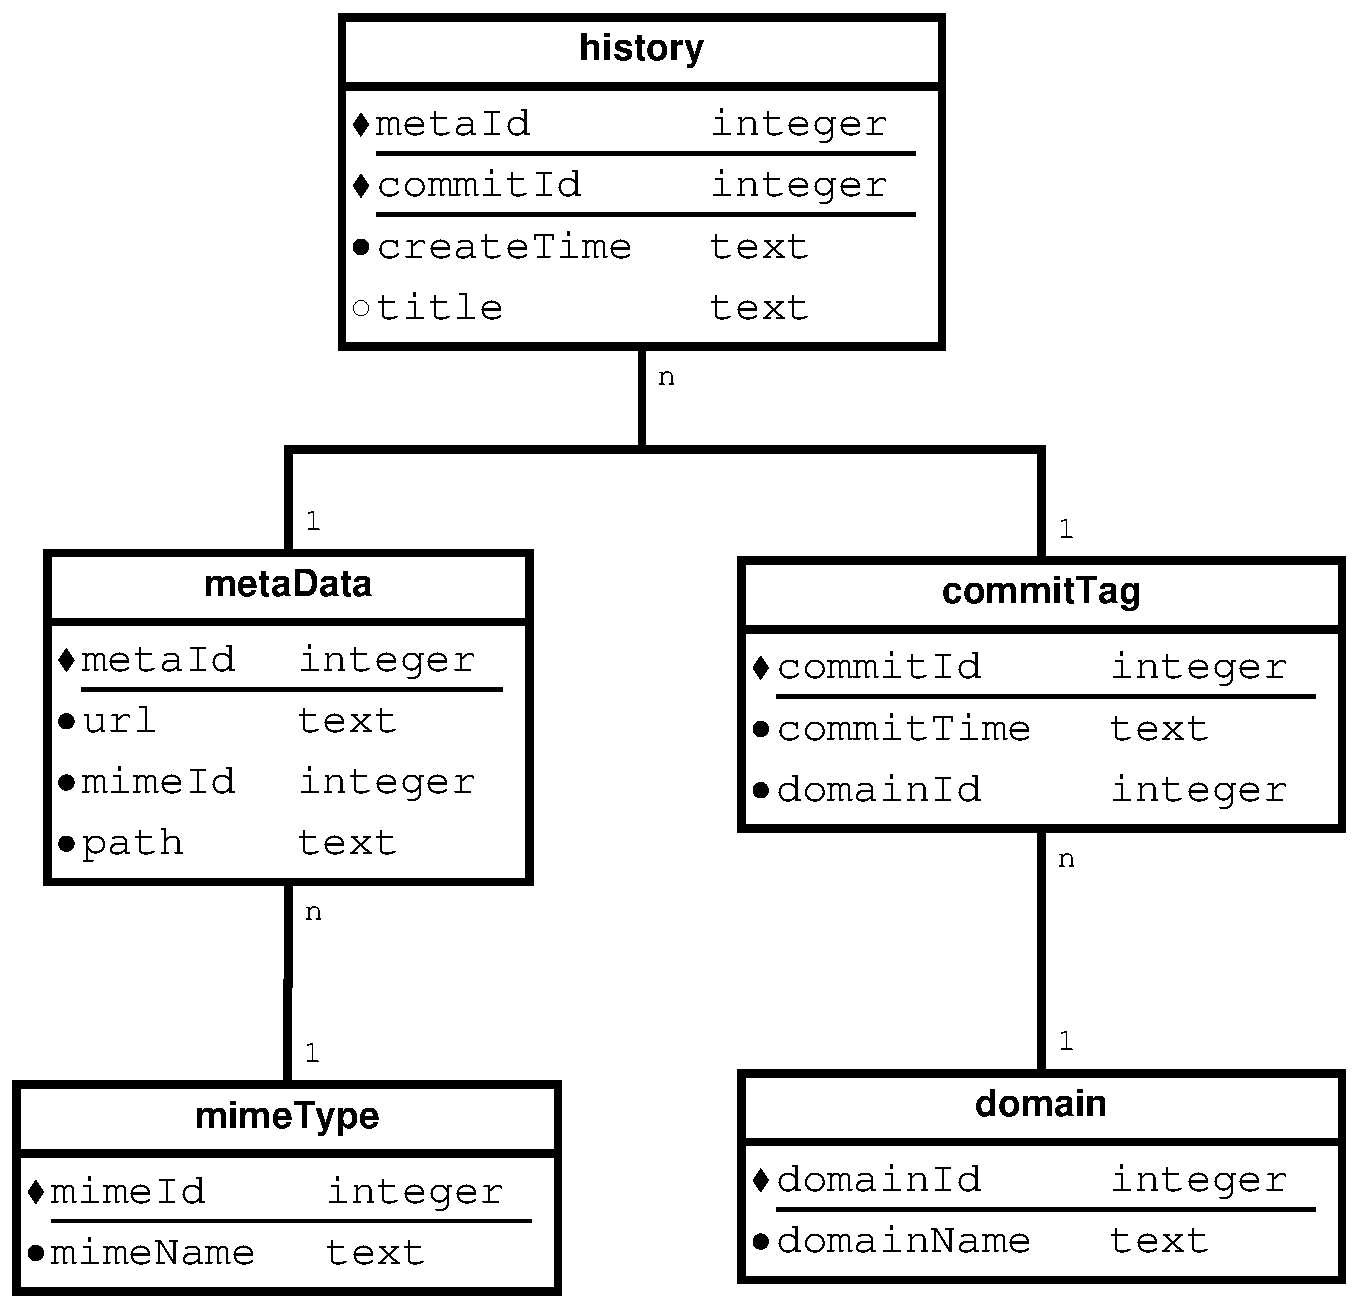
\includegraphics[width=0.6\textwidth]{design/data/db.eps}
	\caption{Datenbankdiagramm}
\end{figure}

\section{XML-Schema}
Folgendes Skripting des XML-Schemas \ref{req:Xm:schema} zeigt den Aufbau der XML-Datei:
\lstinputlisting[language=XML,basicstyle=\ttfamily\fontsize{8}{10}\selectfont]{../xml/file.xsd}
\subsection{Metadaten}
\ref{req:Xm:content:meta}
Um die Metadaten kompakter und besser lesbar zu gestalten, 
werden diese als Attribute ausgeführt. 
Dabei wird auch die 1:n-Beziehung von commitTag zu Metadaten berücksichtig:
Die commit-Daten bilden ein Unterelement von ,,meta'' und sind in diesm ebenfalls als
als Attribute enthalten.
Damit ist der commitTag auch leichter auslesbar.


Die Metadaten erfassen immer den gesamten Zustand innerhalb der Version (bzw. zu einem CommitTag)
\subsection{Daten}
\ref{req:Xm:content:data}
Das ,,data''-Element ist anfangs immer leer, kann aber durch Benutzer mittels der API-Schnittstellen 
um weitere Elemente erweitert.
Dabei ist auch das XSD-Schema entsprechend dem auskommentierten template zu erweitern.
Der Name des umschließenden Elements muss dabei einmalig sein.

Folgendes Listing zeigt ein Beispiel XML mit leerem data-Knoten:
\lstinputlisting[language=XML,basicstyle=\ttfamily\fontsize{8}{10}\selectfont]{../xml/example.xml}

\section{Klassen}
Diagramm \ref{design:dia:data:db} zeigt die Umsetzung des Modells in Klassen.
Aufgrund der 1:n-Beziehung (siehe oben) von Metadaten und CommitTags sind die entsprechenden
Klassen auch getrennt. 

Damit ist es auch möglich speicherintern CommitTags in Metadaten wiederzuverwenden.
Außerdem werden die CommitTags zur Benachrichtigung der Clients durch den Notifier benötigt.


Die TimeStamp-klasse dient zur Vermittlung zwischen der textbasierten Speicherung von Datumswerten und der
programmierspracheninternen Darstellung z.B. java.util.Date.

Analog zu den XML-Daten enthält ein Metadatenobjekt immer den gesamten Zustand einer Datei zu einem CommitTag.

\begin{figure}[h]
	\centering
	\label{design:dia:data:db}
	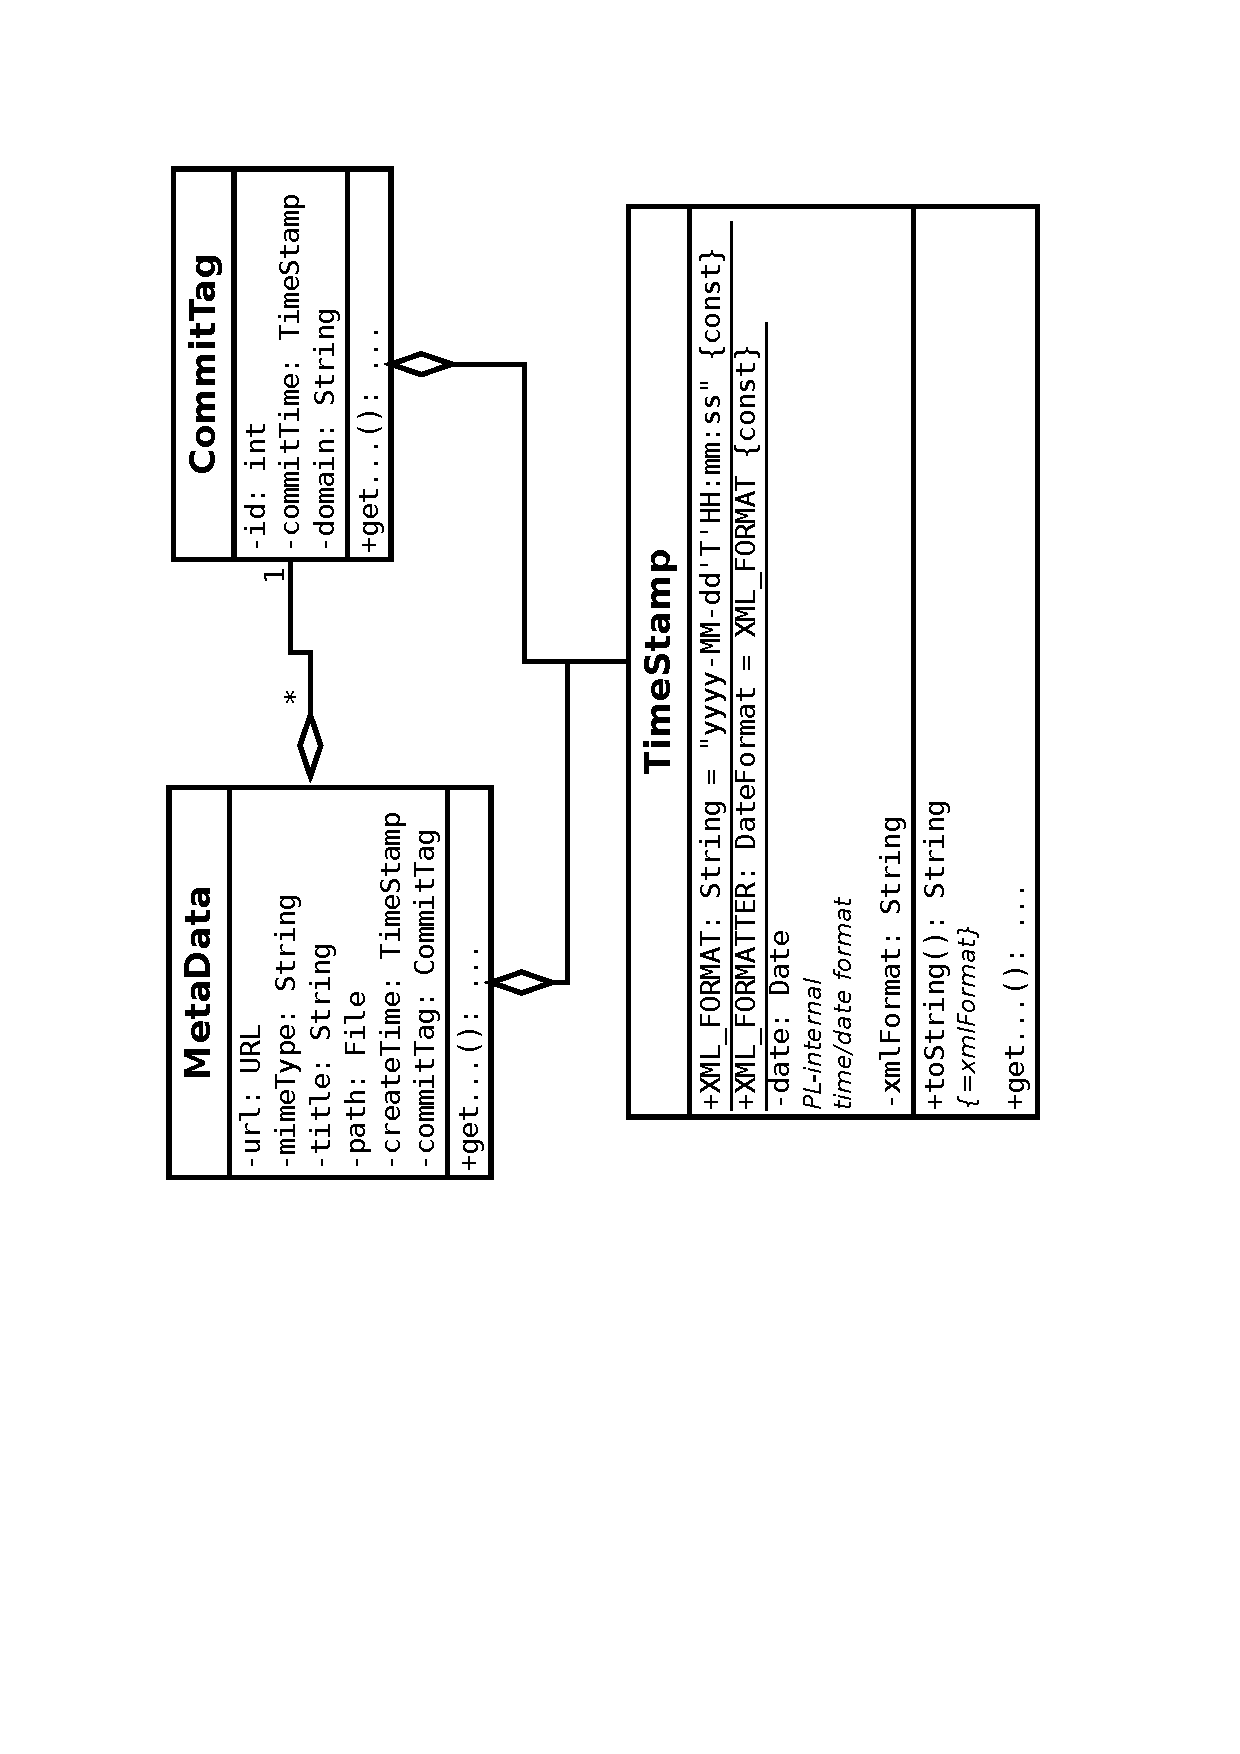
\includegraphics[width=0.6\textwidth, angle=270]{design/data/model.pdf}
	\caption{Datenbankdiagramm}
\end{figure}


\chapter{Backend}
\label{cha:backend}
Das Backend bezieht sich auf den in Python geschriebenen Teil, welcher
öffentlich nicht zugreifbar ist.
Im folgenden werden die zentralen Module aufgelistet, welche in eine
Beschreibung ihrer Funktion, einer Schnittstellenbeschreibung sowie
teilweise einer Begründung aufgeteilt sind.
Die Schnittstellenbeschreibungen sind dabei in englisch kommentierten Python Methoden-Beschreibungen gefasst. 

\section{Testfälle}
Als Testmethode werden Unit-Tests herangezogen, die mit dem bei Python mitgelieferten Frameworks \texttt{unittest}
ausgeführt werden können. Dabei enthält jedes File den dazugehörigen Testcode, welcher durch direktes Aufführen des
.py files ausgeführt wird:

\begin{lstlisting}[language=Python]
# Eigentlicher Source
class XYZ:
    def DoSomething(self, param):
        ...

# Abgetrennter Testcode
if __name__ == '__main__'
   import unittest

   class TestXYZ(unittest.TestCase):
       def TestDoSomething(self):
           ...

   unittest.main()
\end{lstlisting}

\newpage
\section{Programmablauf} 
\label{sec:programmablauf}
\begin{figure}[h!]
\centering
\label{dia:design:backend:overview}
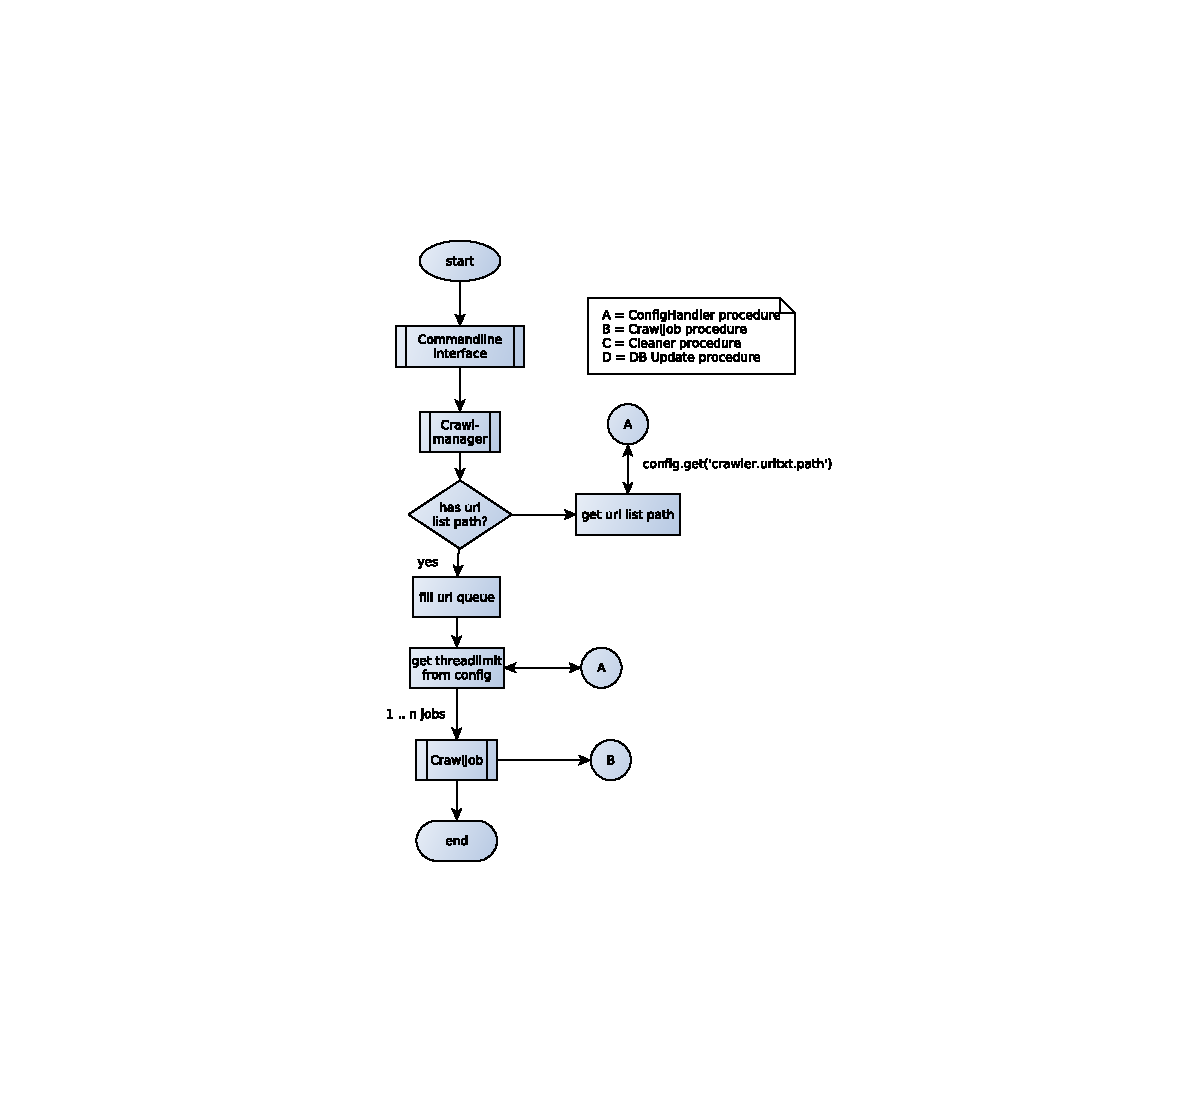
\includegraphics[width=\textwidth]{design/backend/gfx/backend_procedure.eps}
\caption{Ablaufprozedur Backend}
\end{figure}

% section programmablauf (end)

\newpage
\section{Zentrale Module} 
\label{sec:zentrale_module}

\subsection{ConfigHandler}

\paragraph{Ablauf:}
\label{par:ablauf_}
Grundlegender Ablauf beim Lesen von Configwerten:
\begin{figure}[h!]
	\centering
	\label{dia:design:backend:overview}
	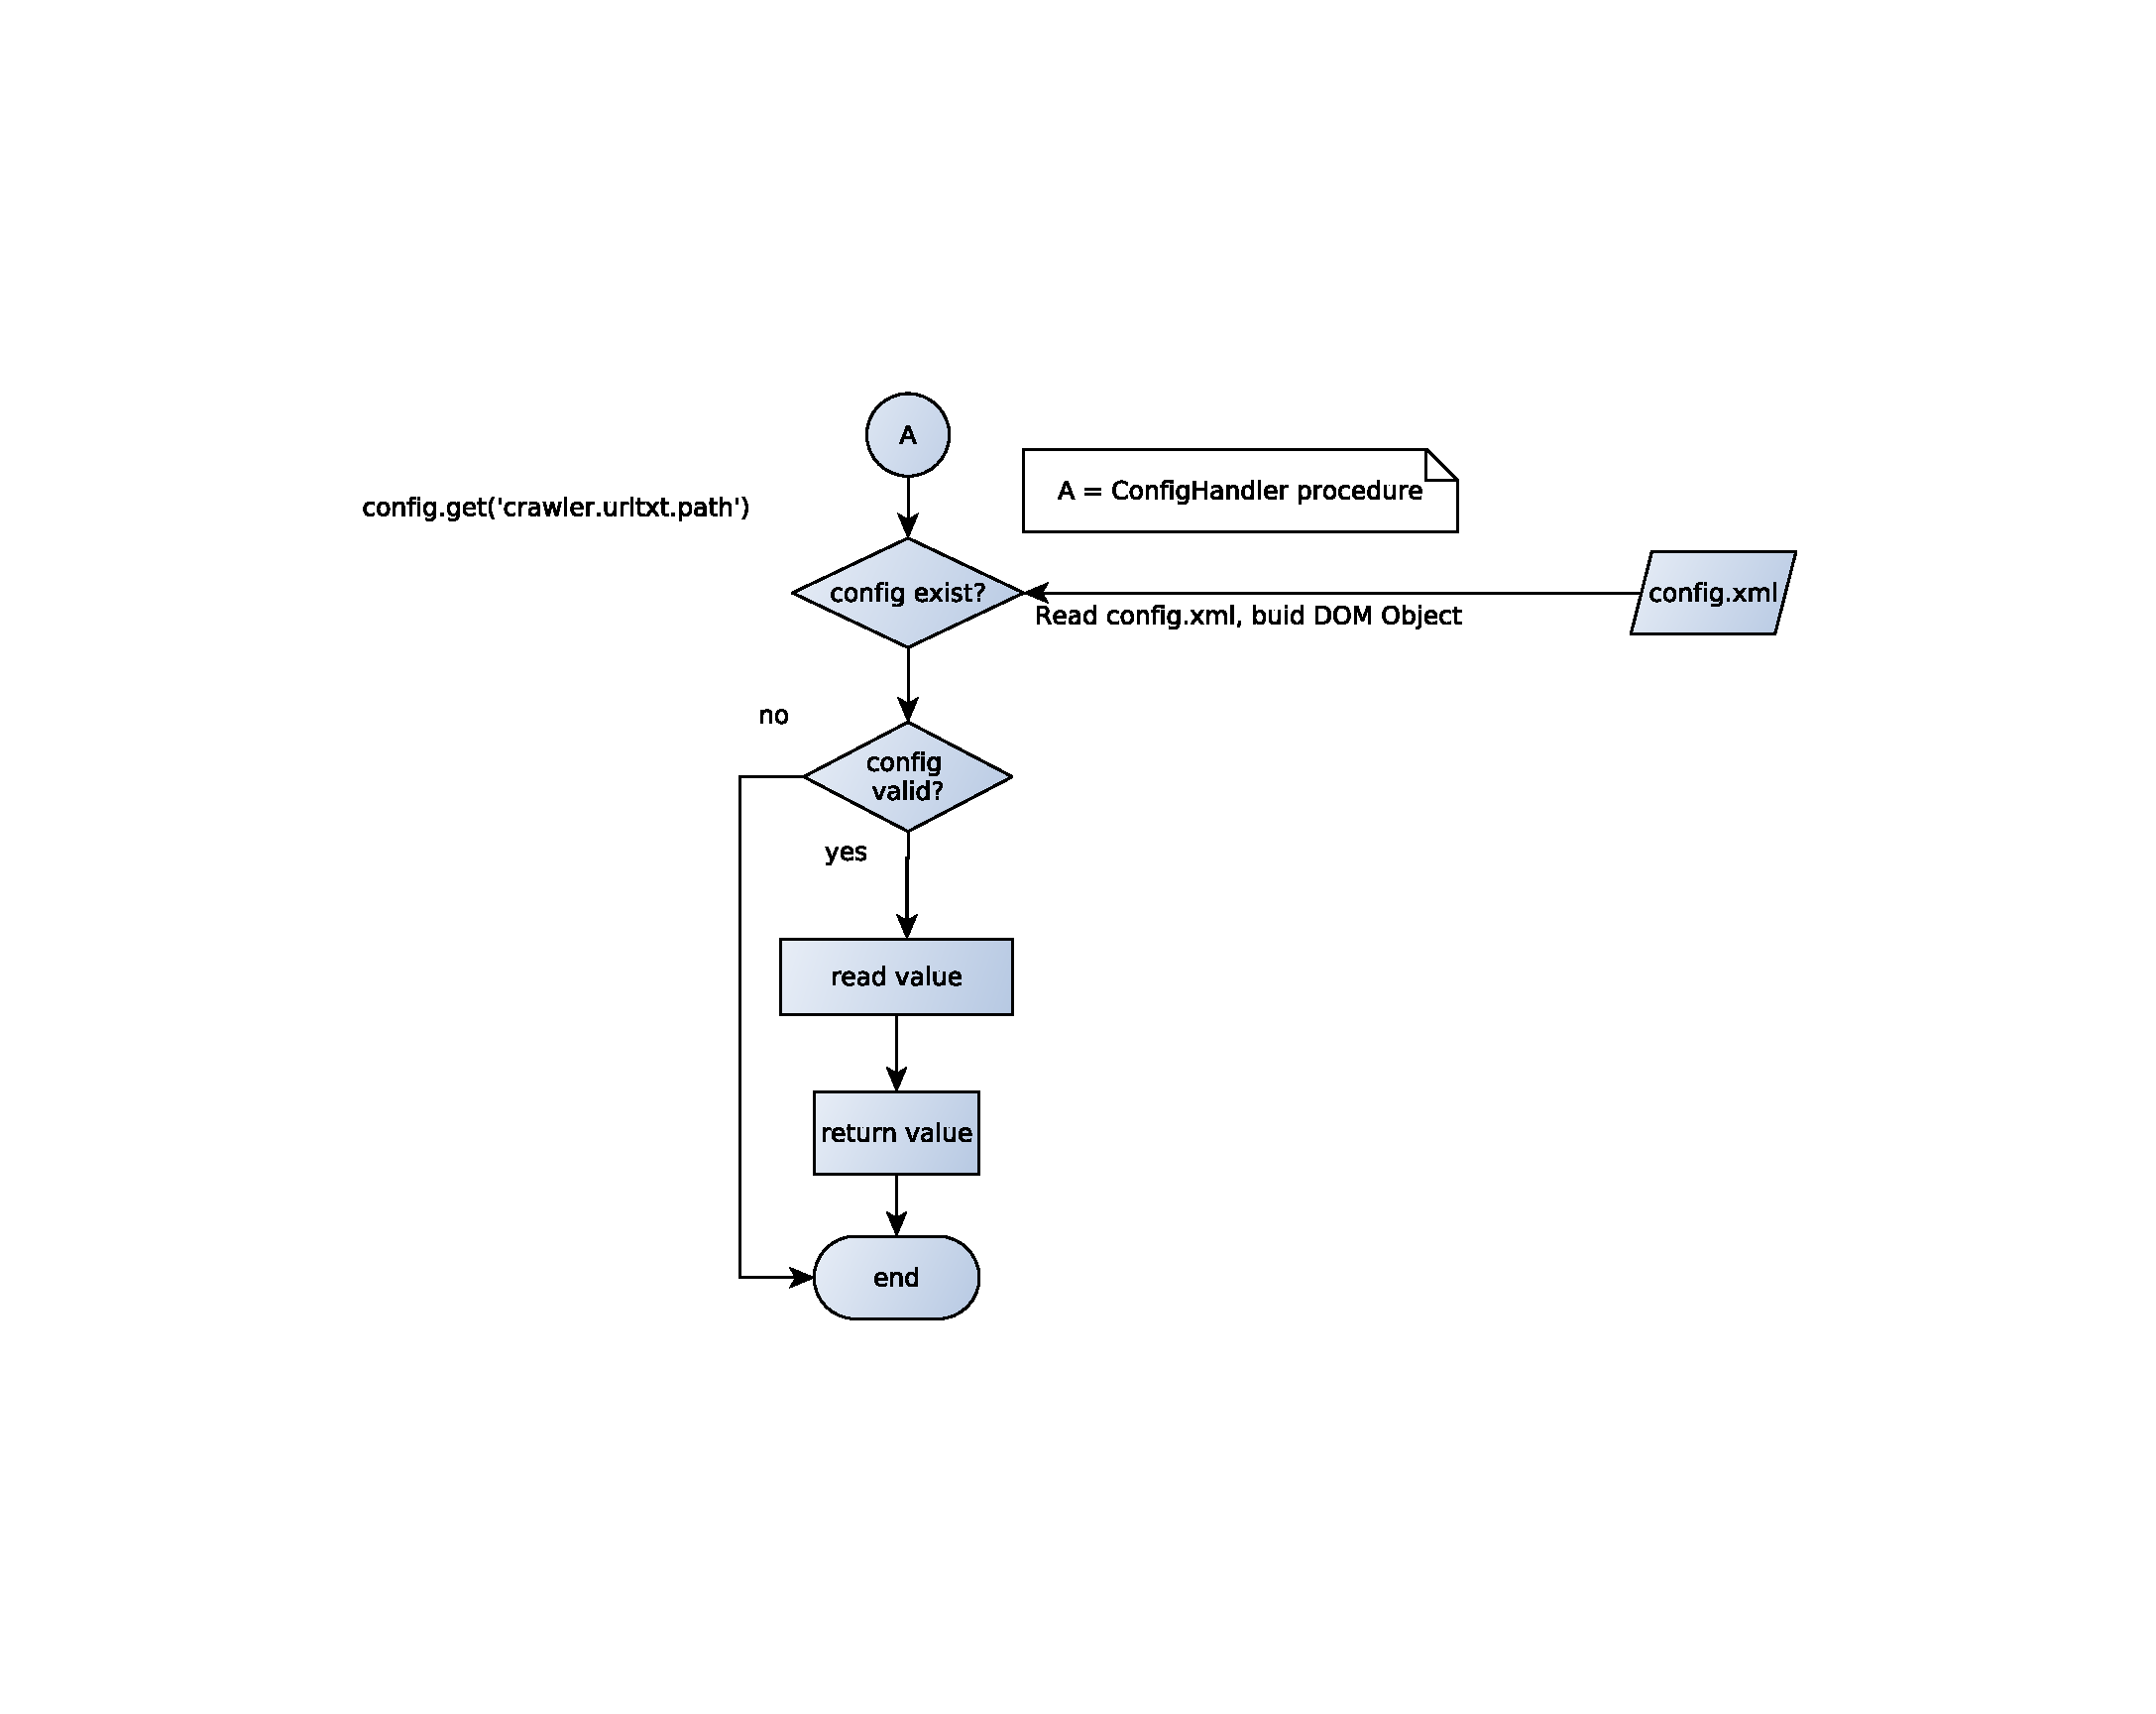
\includegraphics[width=\textwidth]{design/backend/gfx/getting_value.eps}
	\caption{Werte aus der Konfigurationsdatei holen}
\end{figure}

% paragraph ablauf_ (end)
\paragraph{Beschreibung:}
(Entsprechend: \ref{spec:conf})
\label{par:beschreibung_}
Dieser wird zum Lesen und Setzen der Konfigurationswerte verwendet. Die Konfigurationsdatei ist in 
Xml geschrieben und hat folgenden Aufbau:
    \lstinputlisting[language=XML,basicstyle=\ttfamily\fontsize{8}{10}\selectfont]{../../conf/webarchive.conf.xml}
Der Zugriff auf bestimmte Werte ist nach Domainprinzip aufgebaut, so
lässt sich der Wert ,,Serverport'' über eine Punkt-separierte ,,URI'' auslesen: \texttt{webarchive.server.port} 
\\ \\
Der erste Knoten \texttt{webarchive} ist stets vorhanden, und kann daher optional ausgelassen werden.

\begin{figure}[h]
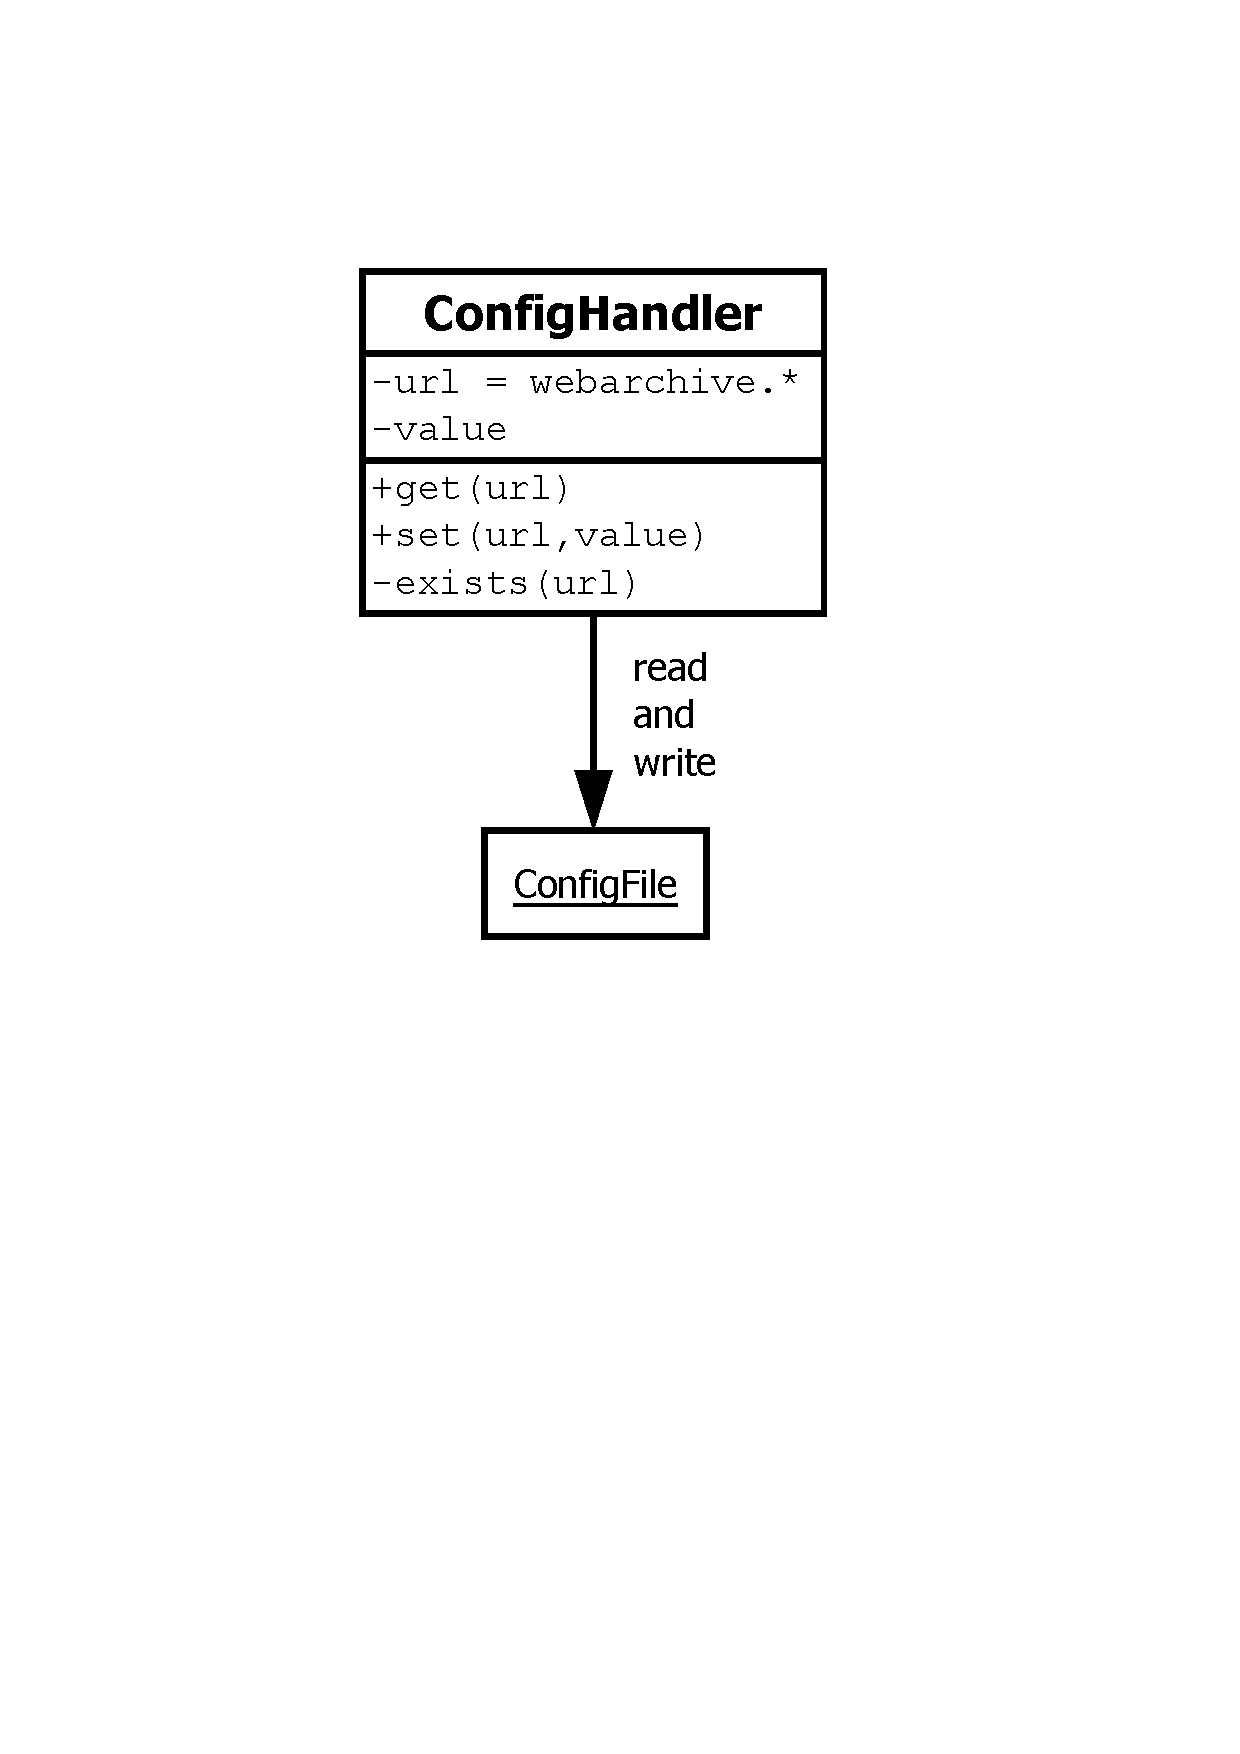
\includegraphics[width=0.6\textwidth]{design/backend/gfx/ConfigHandler.pdf}
\label{sub:confighandler}
\caption{Grobe Übersicht über den ConfigHandler}
\end{figure}

\paragraph{Begründung/Hintergrund:}
\label{par:begr_ndung}
Das relativ einfache URI Prinzip wurde gewählt um stets einen direkten
Bezug zwischen der XML Struktur und den abgefragten Werten herzustellen.
\\
In späteren Versionen ist folgende Erweiterun denkbar: Statt die
Default-Werte fest in den Programmcode zu legen, wird eine systemweite
und immer verfügbare config.xml angelegt, auf die zurückgefallen werden
kann.

% paragraph begr_ndung (end)
\newpage
\subsection{Commandline Interface}
\label{sub:commandline_interface}
\paragraph{Beschreibung}
\label{par:beschreibung}
Dieses Interface realisiert die zentralle Administrationsschnittstelle zum Webarchiv. 
Das Interface soll dabei ähnlich wie git nach dem folgenden Schema funktionieren:
\begin{verbatim}
archive [--general-options] submodule [--arguments-specific-to-submodule]
\end{verbatim}
submodule kann dabei einer der folgenden Module sein:

\begin{table}[H]
\centering
\begin{tabular}{|l|l|}
    \hline
        init & Initialisiert ein leeres archiv an einem bestimmten Pfad \\
    \hline
        crawler & Zugriff auf Starten und Stoppen des Crawlvorgangs \\
    \hline
        javadapter & Starten und Stoppen der Java Schnittstelle \\
    \hline
    db & Bietet Funktionen um die Datenbank neu zu generieren
    (entspricht: \ref{req:Db:recovery}) \\
    \hline
        config & Bietet Zugriff um Werte aus der config zu holen oder zu überschreiben
        (entspricht: \ref{req:Cr:cmd:overwrite}) \\
    \hline
\end{tabular}
\end{table}

\paragraph{Begründung/Hintergrund:}
\label{par:begr_ndung_}
Es wurde sich für ein einfaches Commandline Interface entschieden, da
Kenntnisse im Umgang mit der Unix-Shell auf der User Seite vorrausgsetzt
werden.

% paragraph begr_ndung_ (end)

\subsection{Initialisierung} 
\label{sub:initialisierung}
\paragraph{Beschreibung:}
\label{par:beschreibung}
% paragraph beschreibung (end)
Durch dieses Modul wird ein leerer Archivordner erstellt, der lediglich
ein Default-Configtemplate mit dem Pfad zum Archiv enthält, sowie einen leeren Ordner ,,content'',
in dem später die Crawldaten abgelegt werden.
Weitere Einstellung müssen händisch in der Config nachgetragen werden.
\\
Angelegt wird der Ordner über \texttt{archive init /pfad/zum/archive}.
\paragraph{Schnittstelle:}
\label{par:schnittstelle}
\hfill
\begin{lstlisting}[language=python]
def init_archive(path = '.'):
    """
    Initializes empty archive structure with default Config
    at ,,path'' with the following structure:

      archive/
        content/ 
           # empty
        webarchive.config.xml
    """
    pass
\end{lstlisting}

\paragraph{Begründung/Hintergrund:}
\label{par:begr_ndung_}
Das Anlegen des Archiv-Ordners wurde nicht dem Nutzer überlassen, da
Fehler hierbei sich auf die spätere Funktionsweise auswirken können.
% paragraph begr_ndung_ (end)


% paragraph schnittstelle_ (end)
\subsection{Crawlermanager}
\label{sub:crawlermanager}
\paragraph{Beschreibung:}
\label{par:beschreibung_}
% paragraph beschreibung (end)
Der Crawlermanager liest eine Liste mit URLs aus einer Datei, die entweder auf der Kommandozeile oder in
der Config definiert wurde. Die URLs sind in diese Datei zeilenweise einzutragen und können durch ein \# auskommentiert werden.
Über einen ThreadPool wird dann für jede URL ein Crawljob gestartet. Die maximale Anzahl der dabei laufenden Crawljobs wird bei
der Instanzierung des ThreadPools aus der Config gelesen.
\\
Desweiteren hat der Crawlermanager nur administrative Funktionen wie dem Stoppen der laufenden Crawljobs.
\paragraph{Schnittstelle:}
\label{par:schnittstelle_}
Prinzipieller Aufbau des Crawlmanagers:
% paragraph schnittstelle_ (end)
\begin{lstlisting}[language=python]
class CrawlManager:
    def __init__(self):
        """
        Instance a new CrawlerManager,
        which must be started via start()
        """
        pass

    def start(self):
        """
        Reads configured URLs from Config, and start a new job for each
        """
        pass

    def shutdown(self,hard=False): 
        """
        Shuts down currently running crawljobs
        If hard is set to True, currently running jobs
        are canceled immediately, instead of syncing already
        gathered data to archive.
        """
        pass

    def reload(self):
        """
        Reloads configured URLs and replaces current Queue with new URLs.
        Leaves running Jobs untouched.
        """
        pass

\end{lstlisting}

\newpage
% paragraph api_ (end)
\subsection{Crawljob}
\label{sub:crawljob}
\paragraph{Ablauf:}
    Als Programmaublaufplan eine grobe Übersicht:
\label{par:ablauf_}
\begin{figure}[H]
	\centering
	\label{dia:design:backend:overview}
	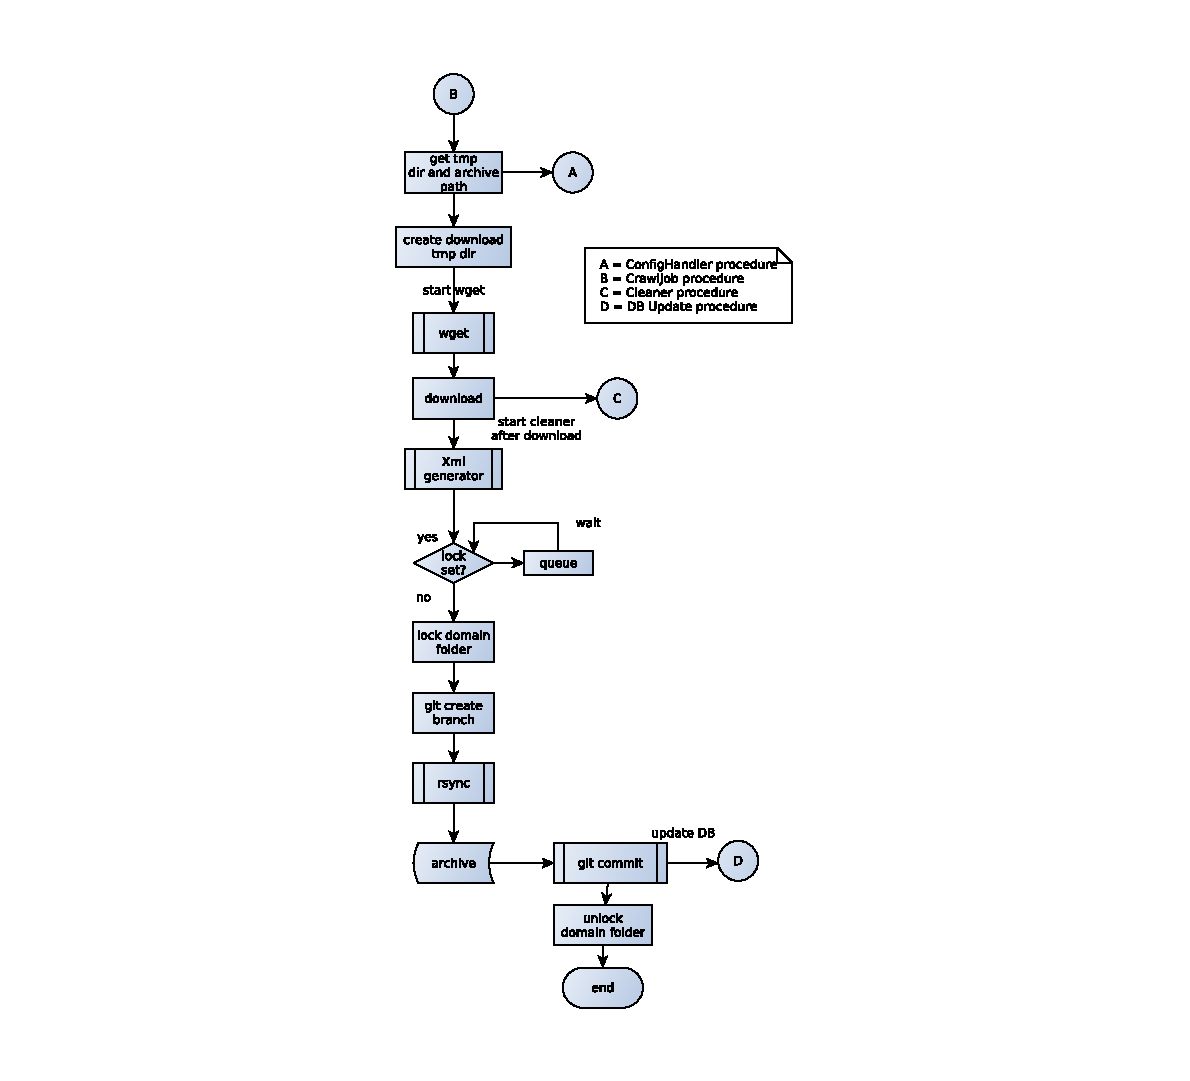
\includegraphics[width=\textwidth]{design/backend/gfx/crawljob.eps}
	\caption{CrawlJob Prozedur}
\end{figure}


% paragraph ablauf_ (end)

\paragraph{Beschreibung:}
\label{par:beschreibung_}
Der Crawljob ist ein autonomer Thread der die unten aufgelisteten Submodule beeinhaltet.
Bevor die einzelnen Submodule abgearbeitet werden, wird ein temporäres Arbeitsverzeichnis angelegt.
Die Lage dieses Verzeichnisses kann in der Config festgelegt werden.
\paragraph{Schnittstelle:}
\label{par:api_}
\hfill

\begin{lstlisting}[language=python]
class CrawlJob():
    def __init__(self, ident, url):
        """
        Gets Identity and Url that should be crawled,
        Identity is needed to generate tmp folder
        """
        pass

    def shutdown(self, hard=False): 
        """
        Shuts down currently running crawljob
        If hard is set to True, currently running job
        is canceled immediately, instead of syncing already
        gathered data to archive.
        """
        pass
\end{lstlisting}
\paragraph{Begründung/Hintergrund:}
\label{par:begr_ndung_hintergrund_}
Ein ,,Wget-Wrapper'' wird zum Crawlen verwendet, da wget alle vom iisys benötigten Funktionalitäten bietet und
in der kürze der Zeit kein gleichwertiger Ersatz implementierbar ist. Um das Crawlen global zu 
beschleunigen wurde dieses ,,paralellisiert'', es werden hier einfach mehrere Wget-Wrapper Instantzen gestartet.
Um die Gesamtgeschwindigkeit des Systems zu steigern wird ebenfalls empfohlen die ,,tmp''-Crawlordner auf ein
ramfs (\footnote{\url{http://wiki.debian.org/ramfs}}) zu legen.

\subsubsection{Wget}
\label{ssub:wget}
\paragraph{Beschreibung:}
\label{par:beschreibung_}
% paragraph beschreibung_ (end)
Eine Managementschicht zur Abstraktion von wget.
Dieser wird eine Domain zugeteilt welche von wget mit konfigurierbaren Parametern gecrawlt wird.
Die allgemeine Webseitenstruktur wird dabei intakt gelassen:

\begin{verbatim}
    www.heise.de/
        index.html
        news/
            newsfeeds.html
            favicon.png
        ...
\end{verbatim}

\paragraph{Schnittstelle:}
\label{par:schnittstelle_}
\hfill
\begin{lstlisting}[language=python]
class Wget():
    def __init__(self, tmpfolder, url):
        """
        Instance a new Wget Wrapper,
        which must be started with start()

        tmpfolder: The folder where the downloaded data will be stored
        url: The url you want to be crawled recursively
        """
        pass

    def start(self): 
        """
        Start crawling the URL in the background,
        the function returns immediately
        """
        pass

    def stop(self):
        """
        Stop a running wget instance
        If start() was not called, or finished already,
        this function is a No-op
        """
        pass
\end{lstlisting}


\newpage
\subsubsection{Cleaner}
\label{ssub:cleaner}
\paragraph{Beschreibung:}
\label{par:beschreibung_}
Der Cleaner bereingt die Verzeichnisstruktur indem er leere Ordner und Dateien löscht.
Desweiteren wird folgende Restrukturierung durchgeführt:
\begin{verbatim}
    www.heise.de/ 
        index.html/
            data
        news/
            newsfeeds.html/
                data
            favicon.png/
                data
        ...
\end{verbatim}


\begin{itemize}
    \item Ordner werden intakt gelassen
    \item Für jede reguläre Datei wird ein gleichnamiges Verzeichnis angelegt
    \item Die regulären Daten werden in dieses Verzeichnis mit den Namen ,,data'' verschoben.
\end{itemize}

Außerdem werden während des Strukturierens die grundlegenden Metadatan als Liste im Speicher gesammelt.
Bevor die Datei an das Filtersystem weitergeleitet wird, wird ein ,,Titel'' abhängig vom MIME-Type ermittelt.
Pro Datei werden die konfigurierten Filter ausgeführt, welche entscheiden ob eine Datei gelöscht werden soll oder nicht.
Gibt ein Filter ,,false'' zurück, so wird der jeweilige Dateiordner samt Inhalt sowie die Metadatan gelöscht,
ohne dass weitere Filter aufgerufen werden müssen.
\\
Die gesammelten Metadaten werden in einem Metadatenobjekt gesammelt. Die gesammelten Daten entsprechen dabei 
der Liste aus \ref{spec:model} abzüglich der ,,commitTime'', da diese erst beim Check-In erhoben wird.
\newpage
\paragraph{Ablauf:}
\label{par:ablauf_}
\hfill
\begin{figure}[H]
	\centering
	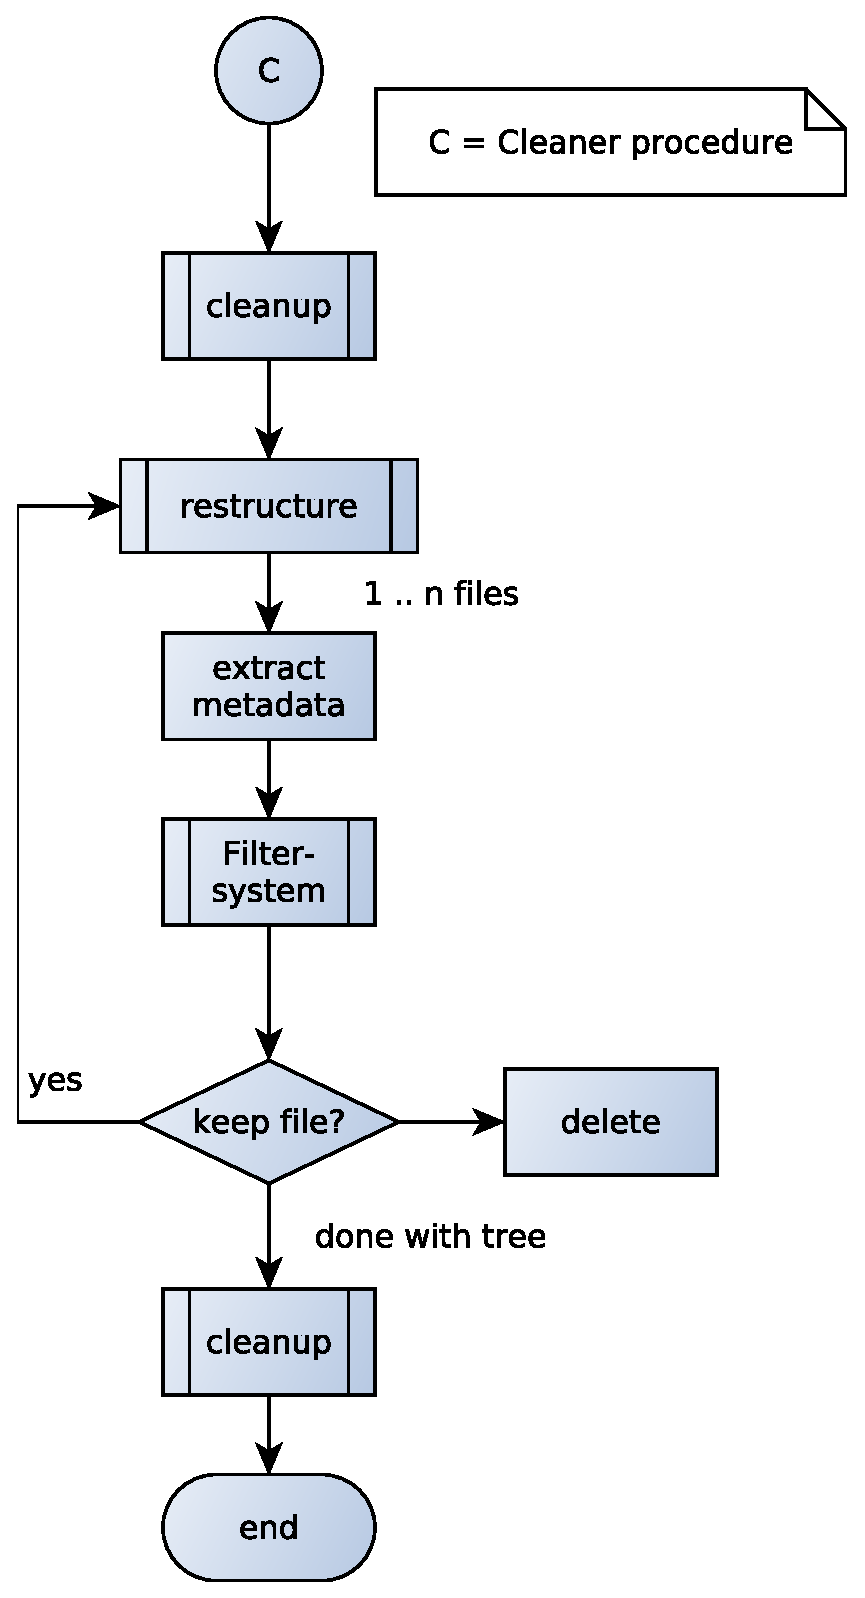
\includegraphics[width=0.5\textwidth]{design/backend/gfx/cleaner.eps}
	\caption{Cleaner Prozedur}
\end{figure}
\paragraph{Schnittstelle:} 
\label{par:schnittstelle_}
\hfill
\begin{lstlisting}[language=python]
class Cleaner():
    def __init__(self, path):
        """
        Instance a new cleaner, which is
        supposed to cleanup recursively in ,,path''
        """
        pass

    def restructure(self): 
        """
        Traverse the filetree and restructure
        it as described above.
        """
        pass
  
    def cleanup(self):
        """
        Remove emtpy files and directories
        in ,,path'' recursively
        """
        pass
\end{lstlisting}

\paragraph{Begründung/Hintergrund:}
\label{par:hintergrund_}
Beim Cleaner wird auf das Unix Tool ,,find'' zugegriffen. Dieses eignet sich aufgrund einer Vielzahl
von Optionen und der Möglichkeit weitere ,,Kommandos'' zu übergeben, gut dazu eine Ordnerstruktur rekursiv
zu durchlaufen und leere Dateien und Ordner zu löschen.

% paragraph hintergrund_ (end)

% paragraph schnittstelle_ (end)
\subsubsection{Filtersystem}
\label{ssub:filtersystem}
\paragraph{Beschreibung:}
\label{par:beschreibung_}
Gemäß \ref{req:Fi:interface} wird ein Filtersystem für gecrawlte Daten
implementiert.

\begin{description}
  \item[Initialisierung] Bei jedem Cleanup-Vorgang werden alle .py files
    aus dem konfigurierte Filter-Verzeichnis in eine Liste eingelesen
  \item[Filtervorgang] Für jede reguläre Datei wird die Liste mit dem
    Filtern durchlaufen. Die einzelnen .py files werden in einem
    Subinterpreter gestartet, und ihnen wird eine Kopie des
    Metadaten-Dictionaries des entsprechenden Files mitgegeben
    \texttt{filter\_input}.
  \item[Auswertung] Jeder Filter bekommt zudem eine Boolean-Variable
    \texttt{filter\_result} übergeben, welche anfangs auf \texttt{True}
    gesetzt ist. Will der Filter die Datei aussortieren so setzt er sie
    auf ein unwahren Wahrheitswert. 
  \item[Aussortierung] Gibt der Filter \texttt{False} zurück, so wird
    das Metadaten-Dictionary, sowie der zugehörige Ordner gelöscht. 
    Bei True wird regulär weitergemacht.
\end{description}

\paragraph{Schnittstelle:}
\label{par:schnittstelle_}
Filter werden während des ,,Cleaner'' Vorgangs ausgeführt.
\begin{lstlisting}[language=python]
    # Inside the filter file two additional global variables
    # are defined:
    #     filter_input  : A copy of a metadata dictionary object
    #     filter_result : The decision of the filter is stored here
    #                     by default the decision is True.
    #
    # Note: filter *.py files cannot be run directly, since 
    #       filter_input and filter_result will not be defined there
    #
    # Example:
    if filter_input['mimeType'] == 'image/gif':
        filter_result = False
\end{lstlisting}
% paragraph schnittstelle_ (end)

\paragraph{Begründung/Hintergrund:}
\label{par:begr_ndung_}
Die Filter werden in Python kodiert, da dies mit einfachem eingebauten Support für
Dictionaries und Subinterpreter eine optimale Lösung darstellt.
Java ist in unsere Augen nicht sinnvoll da einzelne Filter
selten über mehr als 100 Zeilen Quelltext verfügen werden.
% paragraph begr_ndung_ (end)


\subsubsection{Xml Generator}
\label{ssub:xmlgen}
\paragraph{Beschreibung:}
\label{par:beschreibung_}
% paragraph beschreibung_ (end)
Hierbei werden aus der Metadatenliste Xml-Dateien zum jeweiligen Content
geschrieben (\texttt{data.xml}, siehe \ref{spec:xml}) 
Beim Xml generieren werden die Metadaten mit dem aktuellen Systemdatum versehen.
\paragraph{Schnittstelle:}
\label{par:schnittstelle_}
\hfill

\begin{lstlisting}[language=python]
class XmlGenerator:
    def __init__(self, meta_obj):
        """
        Build a data.xml from a template and the meta_obj dictionary
        """
        pass

    def write(self, path = None):
        """
        Write XML to location ,,path'', 
        if not specified the path from meta_obj is taken

        Throws: IOError on failure
        """
        pass
\end{lstlisting}
% paragraph schnittstelle_ (end)
\paragraph{Begründung/Hintergrund:}
\label{par:begr_ndung_hintergrund_}
Um Schreibzugriffe auf die Festplatte (höchstwahscheinlich langsamste Komponente im System) zu minimieren
und nicht doppelt traversieren zu müssen werden die Metadaten nach dem extrahieren im Speicher gehalten und
erst kurz vor dem Synchronisieren ins Archiv generiert und auf die Festplatte geschreieben. 


% paragraph begr_ndung_hintergrund_ (end)
\subsubsection{DB Generator}
\label{ssub:dbgen}
\paragraph{Beschreibung:}
\label{par:beschreibung_}
Analog zur Xml-Generierung wird ein SQL-Statement erstellt, dass Daten aktualisiert oder neu hinzufügt.
Ist die Datenbank noch nicht vorhanden so wird sie neu erstellt.
% paragraph beschreibung_ (end)
\paragraph{Ablauf:}
\label{par:ablauf_}
\hfill
\begin{figure}[H]
	\centering
	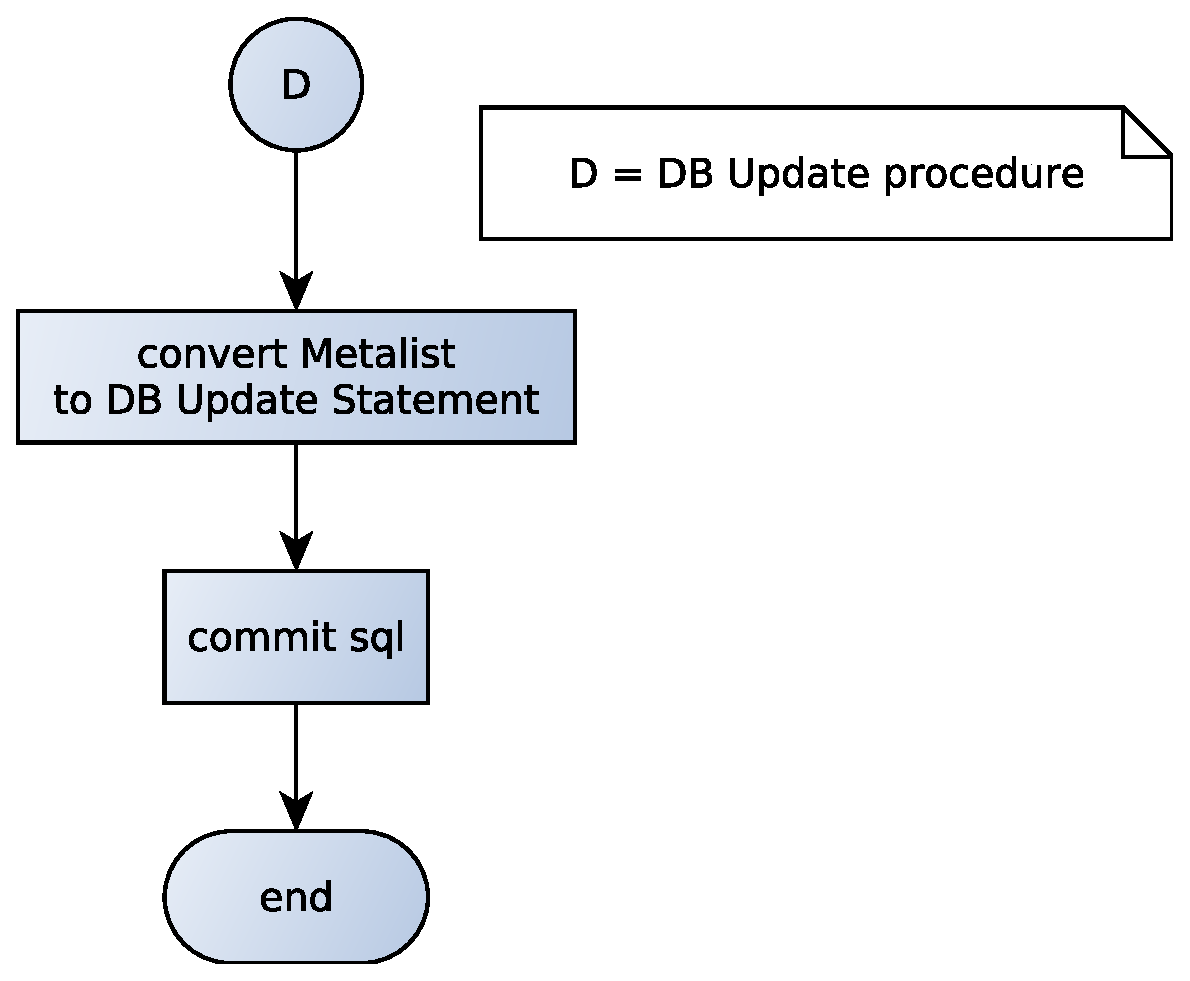
\includegraphics[width=0.5\textwidth]{design/backend/gfx/dbupdate.eps}
	\caption{DB Update Prozedur}
\end{figure}


% paragraph ablauf_ (end)
\paragraph{Schnittstelle:}
\label{par:schnittstelle_}
\hfill
\begin{lstlisting}[language=python]
class DBGenerator:
    def __init__(self, meta_obj_list):
        """
        Build a SQL Query from the meta_obj_list to update and insert new items the Database 
        """
        pass

    def commit(self):
        """
        Send Query to Database,
        this function blocks till finished

        Throws: IOError on failure
        """
        pass
\end{lstlisting}

% paragraph schnittstelle_ (end)

\subsubsection{Rsync}
\label{ssub:rsync}
\paragraph{Beschreibung:}
\label{par:beschreibung_}
Rsync ist eine Managementschicht für das Unix Tool ,,rsync'' \footnote{\url{http://de.wikipedia.org/wiki/Rsync}}. Rsync wird verwendet um die gecrawlten Daten sauber ins Archiv zu synchronisieren.
Hierbei wird der aktuelle gecrawlte Inhalt ins Archiv gespiegelt.
\\
Rsync wird hier direkt auf Systemebene mit folgenden Paramentern ausgeführt:
\begin{figure}[H]
    \centering    
    \texttt{subprocess.call(['rsync','--archive','--checksum','--delete','src','dest'])}
\end{figure}

\begin{itemize}
    \item \texttt{[--archive]}, archive mode
    \item \texttt{[--delete]}, nicht mehr vorhandene Dateien werden im Zielverzeichnis gelöscht
    \item \texttt{[--checksum]}, Dateivergleich basiert auf Checksummen, nicht auf Änderungsdatum
\end{itemize}
aufgerufen um die neu gecrawlten Dateien ins Archiv zu ,,spiegeln''.

\paragraph{Schnittstelle:}
\label{par:schnittstelle_}
\hfill
\begin{lstlisting}[language=python]
class Rsync:
    def __init__(self, path_src, path_dest):
        """
        Instance a new Rsync-Wrapper object,
        which will sync path_src to path_dest
        after calling start_sync() 
        """
        pass

    def start_sync(self):
        """
        Start the synchronisation process,
        this function will block until finished
        """
        pass
\end{lstlisting}

\paragraph{Begründung/Hintergrund:}
\label{par:begr_ndung_hintergrund_}
Rsync wurde gewählt da es sich seit Jahren als Synchronisationstool im Unixbereich bewährt hat.
Da es mit delta files und checksummen arbeitet ist es für den Einsatz eines Archivs optimal.
Durch die Delta-Kodierung/Checksummen wird das Übertragungsvolumen minimiert.

% paragraph begr_ndung_hintergrund_ (end)

\subsubsection{Git}
\label{ssub:git}
\paragraph{Beschreibung:}
\label{par:beschreibung_}
Das Git Modul ist ein Wrapper für das SCM ,,git''. Es wird verwendet um das Archiv mit einer Versionierung auszustatten. Hierzu wird für jeden Crawlvorgang ein Branch erstellt welcher nach der ,,commitTime'' benannt ist. 
Dateien werden in diesen Branch synchronisiert und über ein ,,commit'' bestätigt.

\paragraph{Schnittstelle:}
\label{par:schnittstelle_}
\hfill
\begin{lstlisting}[language=python]
class Git:
    def __init__(self, domain):
        """
        The domain is passed in order to identfiy
        the git-repository on which to operate on
        """
        pass

    def checkout(self, branch_name = None):
        """
        'git checkout' a certain branch-name, or 
        'master' when None is given
        """
        pass

    def branch(self, branch_name):
        """
        Create a new branch named 'branch_name'
        """
        pass

    def commit(self, message = 'edit'):
        """
        Does an 'git add .; git commit -am <message>'
        """
        pass
\end{lstlisting}

\paragraph{Begründung/Hintergrund:}
\label{par:begr_ndung_hintergrund_}
Da die Implementierung eines nativen Python Interface zu git selbst mit GitPython
\footnote{\url{http://gitorious.org/git-python}} oder Dulwich \footnote{\url{http://www.samba.org/~jelmer/dulwich/}}
für die uns zu Verfügung stehenden 6 Wochen zu aufwendig ist, wird die Implementierung über
Python's \texttt{subprocess.call()} Schnittstelle statt finden. Durch den ,,Proof of concept'' können
erste Erfahrungen mit git als Archivierungssystem gesammelt werden und bei Bedarf eine native Implementierung
umgesetzt werden.


% paragraph begr_ndung_hintergrund_ (end)
\subsection{Logger}
\label{sub:logger}
\begin{figure}[H]
    \centering    
    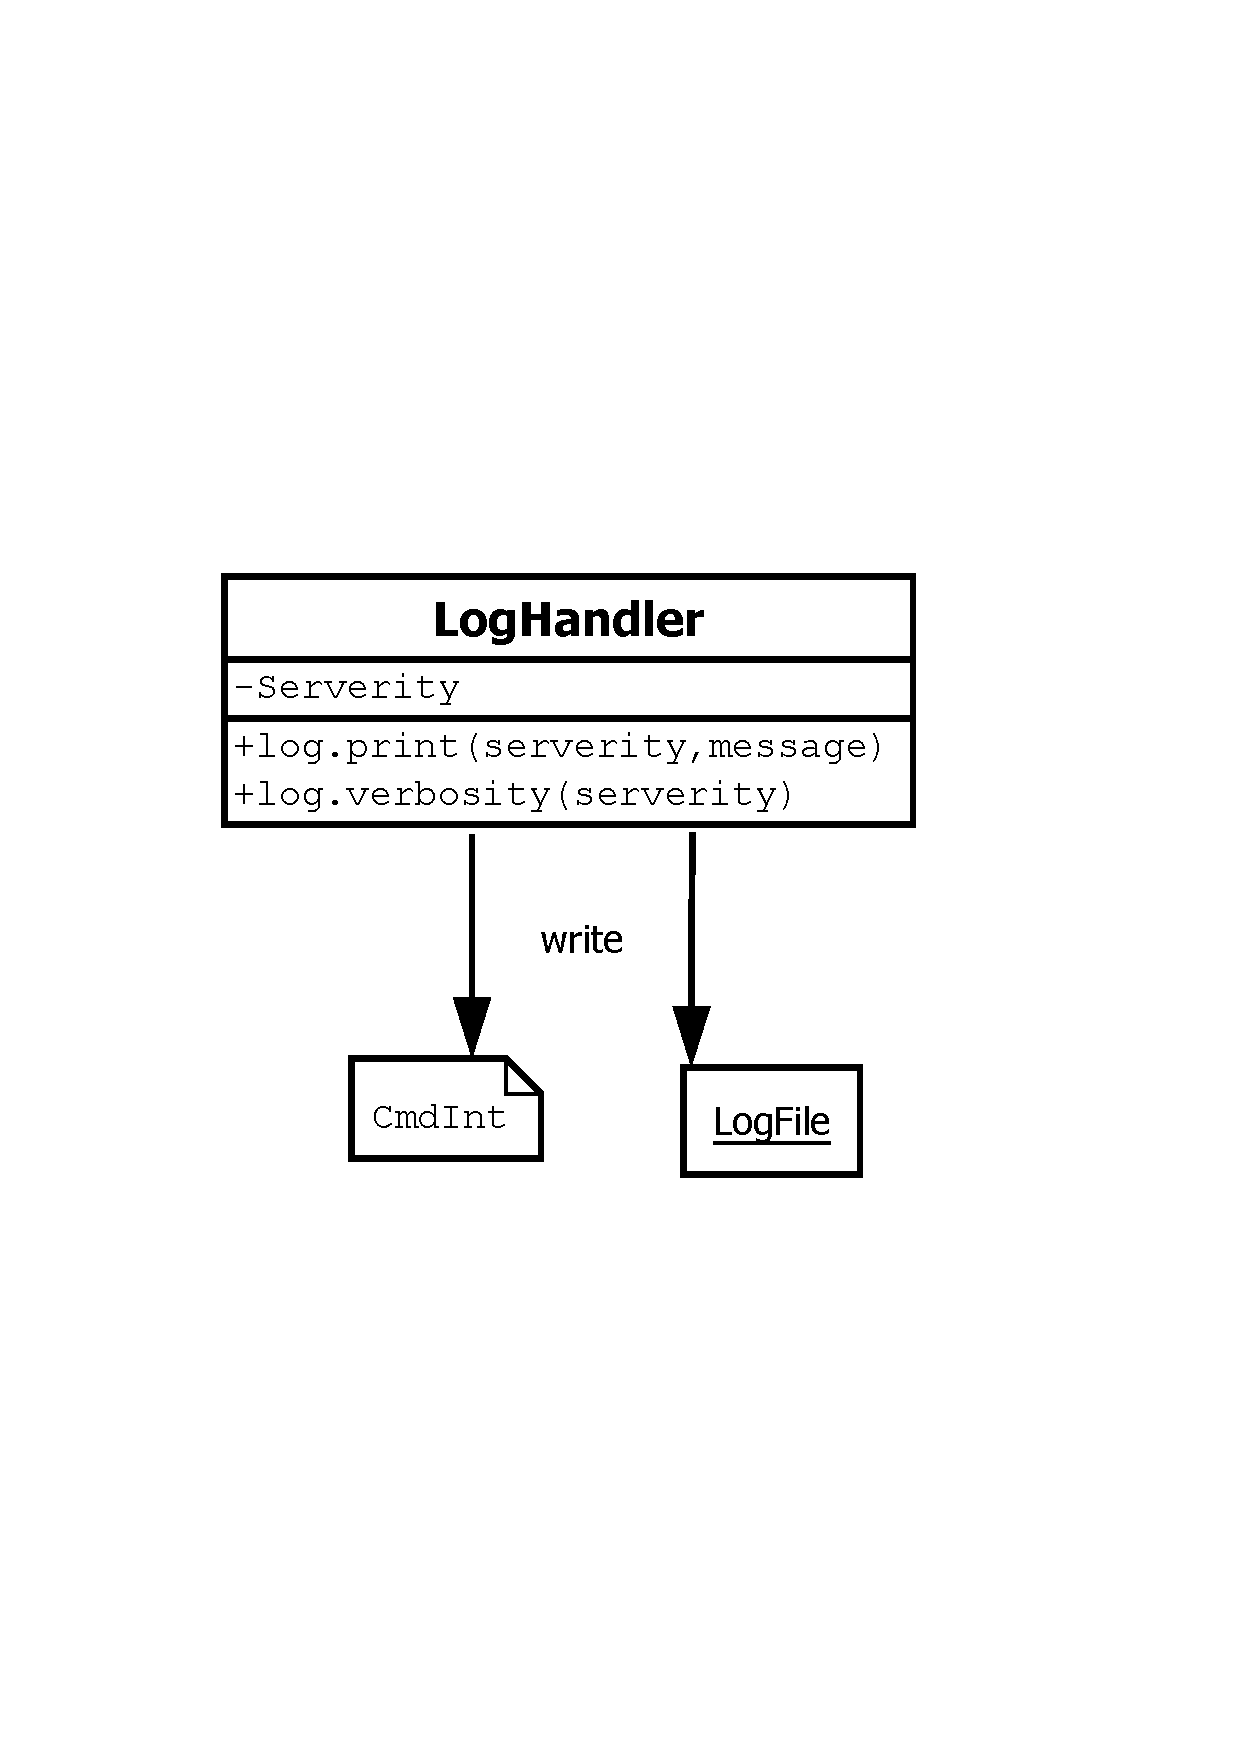
\includegraphics[width=0.6\textwidth]{design/backend/gfx/LogHandler.pdf}
    \caption{Grobe Übersicht über die Logfunktionalität}
\end{figure}

\paragraph{Beschreibung:}
\label{par:beschreibung}

Der Logger wird für das zentrale Loggen im Backend verwendet. Er implementiert die folgenden Error Level:

\begin{table}[h]
\centering
\begin{tabular}{|l|l|}
    \hline
    \texttt{critical} & Schwere unerwartete Fehler \\
    \hline
    \texttt{error} & Fehler aufgrund von fehlerhaften Eingaben \\
    \hline
    \texttt{warning} & Unkritische Fehler \\
    \hline
    \texttt{info} & Allgemeine Statusinformationen \\
    \hline
    \texttt{debug} & Debug-Informationen für Entwickler \\
    \hline
\end{tabular} 
\end{table}
% paragraph beschreibung (end)


\paragraph{Schnittstelle:}
\label{par:schnittstelle_}
Folgende Funktionen werden bereitgestellt:
\begin{lstlisting}[language=python]
def print(severity, *messages):
    """
    Print an Array of messages with a certain severity
    """
    pass

def verbosity(severity):
    """
    Set the verbosity of the program, 

    Passing a severity of 'debug' for example means
    that all messages are printed, while passing 'warning'
    would mean that only Warnings, Errors and Critical Errors 
    are printed.

    This has only effect on terminal output,
    all logmessages will be written to file anyway.
    """
    pass
\end{lstlisting}

\section{Database Recovery} 
\label{sec:database_recovery}
\ref{req:Db:recovery}
Das Recovery-Werkzeug traversiert über alle momentan vorhandenen Domains, und laufen durch alle dort vorhandenen Branches, und traversieren deren 
jeweilige Git-History von hinten nach vorne.
Dabei wird aus den XML Metadaten eine neue Datenbank gebildet.
% section database_recovery (end)

\section{Util} 
\label{sec:util}
\paragraph{Beschreibung:}
\label{par:beschreibung_}
Das Util Modul stellt verscheidene Funktionen die von mehreren Modulen genutzt werden bereit.
Erwähnenswert ist hier der ,,Lockmechanismus''
auf Dateisystemebene um Daten beim Zugriff auf gemeinsame  Ressourcen zu schützen.

\paragraph{Schnittstelle:}
\label{par:schnittstelle_}
\hfill
\begin{lstlisting}[language=python]
    def lock(domain_path):
        """
        Create a lockfile in domain, if already
        being blocked wait till it is unlocked

        Returns: true if lock could be acquired, false on failure
        """
        pass

    def try_lock(domain_path):
        """
        As lock(), but return immediately when locking is not possible,

        Returns: true on success, false on already locked domain
        """
        pass

    def unlock(domain_path):
        """
        Unlocks previously created Lock, does nothing if not already locked.

        Returns: true if a lock was removed, false if none was found
        """
        pass
\end{lstlisting}



\section{Javadapter} 
\label{sec:javadapter}
\paragraph{Beschreibung:}
\label{par:beschreibung_}
Der ,,Javadapter'' stellt eine Schnittstelle zwischen Python und Java dar.
\begin{description}
  \item [Daemon] Er ist als Daemon implementiert, und ist über einen
    definierten Hostname und konfigurierbaren Port erreichbar 
    (Standardmäßig: \texttt{localhost:42421})
  \item [Kommunikation] Jegliche Interaktion erfolgt über ein
    zeilenbasiertes Textprotokoll. Der Client (Hier: Der Java-Server)
    sendet definerte Kommandos, welche mit mit einer Antwortzeile
    und einem abschließenden ,,OK'' oder ,,ACK [FehlerNachricht]''
    beantwortet werden.
  \item [Instanziierung] Der Adapter ist als eigenes Python Modul
    implementiert, und kann über das Commandline-Interface gestartet
    werden.
\end{description}
 
Folgende Kommandos sollen dabei implementiert werden:
Alle Kommandoes nehmen zusätzliche nicht-optionale Argumente die in
eckigen Klammern angegeben sind.
\begin{table}[H]
  \begin{tabular}{|p{4cm}|p{5cm}|p{7cm}|}
    \hline
    \textbf{Kommando} & \textbf{Returnwerte} & \textbf{Beschreibung} \\
    \hline
    \texttt{lock [domain]} 
    & True/False 
    & Lockt eine bestimmte Domain mittels einen Lockfiles 
    \\
    \hline
    \texttt{try\_lock [domain]} 
    & True/False 
    & Wie \texttt{lock}, wartet aber nicht wenn lock bereits gesetzt ist 
    \\
    \hline
    \texttt{unlock [domain]} 
    & True/False 
    & Löscht ein durch \texttt{lock} erzeugtes Lockfile 
    \\
    \hline
    \texttt{checkout [domain] [commitTime]} 
    & Pfad zur ausgecheckten Domain
    & Holt einen alten Stand hervor
    \\
    \hline
    \texttt{commit [domain] [commitTime]} 
    & True/False 
    & Bei Schreibvorgängen müssen die geänderten Dateien
      der Versionverwaltung bekannt gemacht werden.
      Vor einem \texttt{commit} muss ein \texttt{checkout} kommen.
    \\
    \hline
  \end{tabular}
\end{table}

\paragraph{Schnittstelle:}
\label{par:schnittstelle_}
\hfill
\begin{lstlisting}[language=python]
def init_javadapter():
    """
    default way to start javadapter-server,
    listening on a configured port (42421 by default)
    javadapter.lock (including pid) is written to root directory
    """
    pass
def stop_javadapter():
    """
    default way to shutdown javadapter-server,
    releasing lock
    """
    pass
\end{lstlisting}
% paragraph schnittstellen_ (end)

\chapter{Frontend}

\section{Logging und Exceptionhandling}
Bei der Implementierung der Klassen wurde soweit möglich auf das Werfen von Exceptions verzichtet.
Stattdessen wird mit \lstinline{assert}-Statements gearbeitet um ungültige Eingaben, Ausgaben und Zustände schon frühzeitig während der Testphase zu erkennen. 
Diese sind dann später defaultmäßig ausgeschaltet, was die Performance verbessert.

Von Drittanbietern, bzw. der Java-Bibliothek erzeugte Exceptions werden je nach Ursache behandelt.
Interne Fehler werden geloggt und in Logfiles geschrieben. Diese befinden sich ebenfalls im installierten Archivordner.

Von Benutzern verursachte Fehler (z.B. Syntaxfehler in SQL-Klauseln) werden über einen Mechanismus
in der Server-Clientkommunikation zurückgeschickt und im Client erneut geworfen.

\section{Tests}
\subsection{ClientMockup}
	Der ClientMockup testet alle Schnittstellen zum Client, zum Backend (JavaDapter) sowie die Kommunkation übers Netzwerk.
	Dabei wird das Zusammenspiel aller Komponenten getestet.
\subsection{Unittests}
	In den Unittests wird die Funktionalität der einzelnen Klassen getestet.
	Die Tests sind packageweise in Testsuites verknüpft, welche wiederum über eine übergeordnete TestSuite aufgerufen werden können.
	Hier folgt die Erläuterung für paketweise:	
	\subsubsection{webarchive.api}
		In der API werden nur die konkreten Klassen getestet, Schnittstellen
		oder Abstraktionen werden in den konkreten Implementierungen der anderen Pakete oder im ClientMockup getestet.
		\paragraph{.model}
		Bei den Modelklassen müssen hauptsächlich Getter getestet werden.
		Außerdem werden auch illegale Eingaben in die Konstruktoren getestet,
		wobei diese nur mit asserts abgefangen werden, da Objekte später nicht
		ins System geschrieben werden können.
		\paragraph{.select}
		Die API-Selectklassen bereiten die Eingaben der Benutzer auf die
		Select-klassen im Server vor (benannte where-Parameter werden in
		eine generische Arrayform gebracht).

		Es wird deshalb getestet, ob durch Eingaben die richtige Arrayausgabeform erzeugt wird.

		Null-werte sind legal und werden als nicht vorhandene WHERE- bzw. ORDER-BY Klausel interpretiert.
		Das Erkennen von Syntaxfehlern in den Klauseln wird natürlich der Datenbank überlassen.
		\paragraph{.xml}
		Es wird die TagName-klasse getestet, welche dafür sorgt dass Xml-Tagnames mit richtigen Präfixen versehen wird. Es wird also die Erzeugung mit verschieden Eingaben und deren Ausgabe getestet.

	\subsubsection{webarchive.xml}
		Da das XML-Paket hierarchisch aufgebaut ist, sind die Tests dementsprechend gestaltet. 
		In Lowlevel-Klassen werden die Primitivfunktionen getestet, während in den Highlevel-Controllern (XmlHandler, XmlEditor) zusammengesetzte Funktionalitäten getestet werden. 

	Die Netzwerkverbindung wird dabei mit Mockupklassen umgangen. 
	Es wird auch die Konfigurierung von XmlConf mit einer Test-Configdatei geprüft.
	Desweiteren wird geprüft:
	\begin{itemize}
		\item Das Auslesen vorhandener und nicht vorhandener Datenelemente.
		\item Hinzufügen von Datenelementen, inklusive Transformation der DOM und schreiben auf die Festplatte.
		\item Die Übergabe ungültiger Werte wie null, schreibgeschützter oder bereits vorhandener DataElement-objekte, 
		\item Die Validierung: Das Anlegen von neuen Datenelementen, mit hinzugefügten gültigen Elementen in einer Test-xsd-Datei sowie das Hinzufügen invalider Elemente.
	\end{itemize}


	\subsubsection{webarchive.dbaccess}
		Die Datenbankklassen werden mithilfe einer Testdatenbank getestet, welche sich im Ordner \lstinline{test/sql} befindet.

		Bei den Typbezogenen Selects (z.B. SelectMetaDataTest) wird getestet, 
		ob das Mapping zwischen relationeller DB und Objekten funktioniert.
		Außerdem werden erwartete Testwerte aus der Datenbank abgeprüft.
		
		Die abstrakte Klasse SelectJoin wird dahingehend getestet, 
		dass vorbereite SELECT-Statements anhand der übergebenen Parameter richtig zusammengesetzt werden.
		Diese SELECTs werden dann anschließend mit verschiedenen Pseudo-WHERE- und ORDER-BY-Klauseln gefüllt
		und die Syntax geprüft.
		Desweiteren sollen SQL-injections durch interne Abfragen verhindert werden.

		Die Klasse SqlHandler, welche als Fassadenschnittstelle nach aussen dient, wird daraufhin
		geprüft, dass übergeben Select-objekte (aus dem api-package) den richtigen Ausführungsselects zugeordnet werden. Das Ergebnis kann wiederum anhand erwartbar Rückgabewerte geprüft werden.
	\subsubsection{webarchive.server.Server}
		Der Server konnte über UnitTests nur sehr umständlich und unzuverlässig getestet werden, da er im Grunde von allen anderen Modulen und Klassen abhängig ist.
		
		Nach unzähligen Versuchen eine minimalistische Testumgebung für den Server zu schaffen, hat man sich dazu entschieden, die Tests auf den MockupClient auszulagern und keine separaten JUnitTests für ihn zu schreiben.
	\subsubsection{webarchive.client.Client}
		Für den Client wurde ein MockupClient geschrieben, der alle wesentlichen API-Calls aufruft. 
		Da es nur seine Aufgabe ist, Daten an den Server zu schicken und zu empfangen, war das Testen relativ leicht und benötigte auch keine JUnitTestCases, die ohnehin nicht so schnell realisierbar gewesen wären, da der Client auf eine funktionsfähige Serverstruktur angewiesen ist.
		Letztere ginge nicht ohne einen Laufenden Webarchive Crawler, eine Datenbank mit Daten, einem laufenden Javadapter und alle restlichen Java Module.
		Da dies dem Sinn von UnitTests widerspricht, wurde nur auf ein simples API Testen mit einem MockupClient ausgewichen.
	\subsubsection{webarchive.connection.ConnectionHandler}
		Die grundlegende Intelligenz hinter dem Server und Client steckt im ConnectionHandler, der Nachrichten an wartende Threads weiterleitet.
		
		Dieser lässt sich im Gegensatz zum Server und Client direkt testen.
		So wurde ein JUnitTest erzeugt, der zunächst einen ServerConnectionHandler und 1500 Messages mit verschiedenen id's anlegt.
		Anschließend werden 1500 Threads erzeugt, die auf eingehende Nachrichten warten.
		Hiermit wird ein senden und anschließendes warten auf eine Antwort simuliert.
		Nachdem alle 1500 Threads warten, werden weitere 1500 Threads erzeugt die ein wakeUp() auf je eine Nachricht ausführen.
		Sobald ein wartender Thread aufwacht, wird geprüft ob die über wakeUp() zugeordnete Nachricht dieselbe id wie die anfängliche Message hat.
		Zum Schluss joined der Test-Thread allen noch wartenden Threads für maximal 30 sekunden. Wenn diese Zeit überschritten wird, gilt der Test als nicht bestanden.
		Auf der Entwicklermaschine mit nur 2 Kernen und je 2 GHz dauerte der gesammte Vorgang nur wenige sekunden (weniger als 5).
		Damit der Test als erfolgreich gilt, muss die HashMap nachdem alle Threads geweckt wurden leer sein.
		
		Dieser Test wird mehrere Male in verschiedenen Kombinationen ausgeführt.
		Auch ein in der Praxis eher nicht vorkommendes Ereignis, nämlich das Senden von mehreren Antworten direkt hintereinander wurde mit Erfolg getestet.
		
	\subsubsection{webarchive.init.ConfigHandler}
		Der ConfigHandler muss in der Lage sein eine auf der Festplatte liegende XML-Datei einzulesen und einen bestimmten Wert als String wiederzugeben.
		
		Hierfür wurde eine simple XML-Datei als static final String in den Quelltest gepackt und beim setUp des JUnitTests in das aktuelle Verzeichnis geschrieben.
		Anschließend wurden einige Tests bezüglich der Korrektheit der zurückgegebenen Daten gemacht.
		So wurde zum Beispiel getestet ob ein langer XML-Knoten-Pfad wie a.b.c.d.e.f funktioniert, oder beim ausgeben eines übergeordneten Knotens alle sub-Knoten-Inhalte zurückgegeben werden.
		
	\subsubsection{webarchive.server.LockHandler}
		Der LockHandler war genau wie der Server und Client schwer mit JUnit zu testen.
		Allerdings gab es hier die Möglichkeit eine minimalistische Testumgebung zu erzeugen.
		
		Um den LockHandler effektiv zu testen, wurde zunächst ein Javadapter Emulator geschrieben.
		Dieser nimmt eine Verbindung (der echte nimmt viele) an und reagiert ähnlich wie der echte Javadapter auf lock, unlock, commit... Befehle.
		
		Der JavadapterEmu besteht aus dem Verbindungspart in der Klasse selbst und dem EmuHandler, der auf die Befehle regiert und prüft. 
		Bei einem Fehler wird eine Exception an den LockerHandlerTest wieder gereicht.
		
		Für alle Kernbefehle wurden verschiedene Tests geschrieben. 
		Zum einen werden absichtlich nicht vorhandene Domains gelockt, was einen Fehler verursachen MUSS.
		Zum anderen wird geprüft ob der LockHandler mit inkorrekter Anzahl an Parametern zurechtkommt.
	\subsubsection{webarchive.server.FileHandler}
		Der FileHandler muss Dateien von der Festplatte lesen und auf sie schreiben können.
		Auch muss er alle nicht versteckten Dateien in einer Ordnerstruktur anzeigen können.
		
		Hierzu werden vor jedem Test mehrere Ordner und Dateien angelegt.
		
		Anschließend wird mit ein paar simplen Tests die Richtigkeit der geschriebenen und gelesenen Daten überprüft.
		
	\subsubsection{webarchive.server.ServerTestSuite}
		Die Tests der Klassen ConnectionHandler, ConfigHandler, LockHandler und FileHandler sollten über die ServerTestSuite ausgeführt werden.
		Zu beachten ist, dass die ServerTestSuite im Gegensatz zu den anderen Tests des dbaccess,xml,etc. mit deaktivierten Assertions ausgeführt werden muss, da beim initialisieren von einigen temporär erzeugten Klassen ansonsten null werde nicht zugelassen werden.
		Diese assertions sind allerdings nur für den normalen Betrieb gedacht und nicht für das Testen von einzelnen Modulen.
		
\end{document}

